%%%%%%%%%%%%%%%%%%%% author.tex %%%%%%%%%%%%%%%%%%%%%%%%%%%%%%%%%%%
%
% sample root file for your "contribution" to a contributed volume
%
% Use this file as a template for your own input.
%
%%%%%%%%%%%%%%%% Springer %%%%%%%%%%%%%%%%%%%%%%%%%%%%%%%%%%


% RECOMMENDED %%%%%%%%%%%%%%%%%%%%%%%%%%%%%%%%%%%%%%%%%%%%%%%%%%%
\documentclass[graybox]{svmult}

% choose options for [] as required from the list
% in the Reference Guide

\usepackage{mathptmx}       % selects Times Roman as basic font
\usepackage{helvet}         % selects Helvetica as sans-serif font
\usepackage{courier}        % selects Courier as typewriter font
\usepackage{type1cm}        % activate if the above 3 fonts are
                            % not available on your system
%
\usepackage{makeidx}         % allows index generation
\usepackage{graphicx}        % standard LaTeX graphics tool
                             % when including figure files
\usepackage{multicol}        % used for the two-column index
\usepackage[bottom]{footmisc}% places footnotes at page bottom

% see the list of further useful packages
% in the Reference Guide

\makeindex             % used for the subject index
                       % please use the style svind.ist with
                       % your makeindex program

%%%%%%%%%%%%%%%%%%%%%%%%%%%%%%%%%%%%%%%%%%%%%%%%%%%%%%%%%%%%%%%%%%%%%%%%%%%%%%%%%%%%%%%%%


\usepackage{amsmath,amssymb,amsfonts,stmaryrd}
\usepackage{color}
\usepackage{listings}
\lstset{
   basicstyle=\scriptsize\ttfamily,
   %frame=single,
   breaklines=true,
}
\usepackage{hyperref}
\usepackage{tikz}
\usetikzlibrary{arrows}
\usepackage{algorithm}
\usepackage{algpseudocode}
\usepackage[T1]{fontenc}

\newcommand\for{\mathbin{\text{for}}}
\newcommand\inhibits{\mathbin{-\!\Yleft}}
\newcommand\activates{\rightarrow}

\newcommand{\ra}{\rightarrow}
\newcommand{\lra}{\longrightarrow}


\usepackage{bm}
\newcommand{\op}[1]{\mathbf{\ensuremath{#1}}}
\newcommand{\vct}[1]{\bm{#1}}
\newcommand{\cl}[1]{\mathcal{#1}}
\newcommand{\pprob}{\mathit{prob}}

\usepackage{stackrel}
\newcommand{\raf}[1]{\ {\displaystyle\stackrel{\stackrel{#1}{}}{\longrightarrow}}\ }
\def\ra{\longrightarrow}
\newcommand{\laf}[1]{\ {\displaystyle\stackrel{\stackrel{\longleftarrow}{}}{#1}}\ }
\def\la{\longleftarrow}
\newcommand{\rlaf}[2]{\ {\displaystyle\stackrel[{#2}]{#1}{\stackrel{\longrightarrow}{\longleftarrow}}}\ }
\def\rla{\longlefrighttarrow}
%\newtheorem{definition}{Definition}
%\newtheorem{thm}{Theorem}
%\newtheorem{prop}{Proposition}
%\newtheorem{example}{Example}
%\newenvironment{proof}{\vspace{2mm} \noindent {\bf Proof.}}{\hfill $\Box$}
\def\D{{\cal D}}
\def\s{{\vct s}}
\def\sp{{\vct {s'}}}
\def\ddt{{\frac{d}{dt}}}
\def\M{{\cal M}}
\def\S{{\cal S}}
\def\Rob{{\cal R}}
\def\Rlin{\mathbb{R_{\mbox{lin}}}}
\def\Real{\mathbb{ R}}
\def\N{\mathbb{ N}}
\def\Z{\mathbb{ Z}}
\def\I{\mathbb{ I}}
\def\true{\mathit{true}}
\def\false{\mathit{false}}
\def\E{{\bf E}}
\def\A{{\bf A}}
\def\F{{\bf F}}
\def\G{{\bf G}}
\def\X{{\bf X}}
\def\U{{\bf U}}
\def\W{{\bf W}}
\def\R{{\bf R}}
\def\EF{{\bf EF}}
\def\EG{{\bf EG}}
\def\EX{{\bf EX}}
\def\EU{{\bf EU}}
\def\ER{{\bf ER}}
\def\AF{{\bf AF}}
\def\AG{{\bf AG}}
\def\AX{{\bf AX}}
\def\AU{{\bf AU}}
\def\AR{{\bf AR}}


\DeclareMathOperator{\Set}{Set}
%%%%%%%%%%%%%%%%%%%%%%%%%%%%%%%%%%%%%%%%%%%%%%%%%%%%%%%%%%%%%%%%%%%%%%%%%%%%%%%%%%%%%%%%%

\begin{document}

\title*{Lecture Notes MPRI C2-19:\\
Computational Methods for Systems and Synthetic Biology}
% Use \titlerunning{Short Title} for an abbreviated version of
% your contribution title if the original one is too long
\author{Fran\c{c}ois Fages} % and Name of Second Author}
% Use \authorrunning{Short Title} for an abbreviated version of
% your contribution title if the original one is too long
\institute{Fran\c{c}ois Fages \at Inria Saclay Ile de France, 1 rue Honor\'{e} d'Estienne d'Orves, Campus de l'\'{E}cole Polytechnique 
91120 Palaiseau, France, \email{Francois.Fages@inria.fr}
%\and Name of Second Author \at Name, Address of Institute \email{name@email.address}
}
%
% Use the package "url.sty" to avoid
% problems with special characters
% used in your e-mail or web address
%
\maketitle

\abstract{Systems Biology aims at elucidating the high-level functions of the cell from their biochemical basis at the molecular level. A lot of work has been done for collecting genomic and post-genomic data, making them available in databases and ontologies, building dynamical models of cell metabolism, signalling, division cycle, apoptosis, and publishing them in model repositories. In this course we review different computational methods applied to biological systems modelling. We focus on cell processes at the unicellular level which constitutes most of the work achieved in the last two decades in the domain of Systems Biology. We show how rule-based languages and logical methods have played an important role in the study of molecular interaction networks and of their emergent properties responsible for cell behaviours. In particular, we present some results obtained with SAT and Constraint Logic Programming solvers for the static analysis of large interaction networks, with Model-Checking and Evolutionary Algorithms for the analysis and synthesis of dynamical models, and with Machine Learning techniques for the current challenges of infering mechanistic models from temporal data and automating the design of biological experiments.}

\tableofcontents

\newpage

\section{Introduction}
\label{intro}

\hfill\emph{``All life is problem solving'', Karl Popper.}\\

In the early history of Computer Science, the biological metaphor played an important role
in the design of the first models of computation based on neural networks and finite state machines.
The Boolean model of the behaviour of nervous systems given by McCulloch and Pitts in 1943
turned out to be the model of a finite state machine \cite{MP43bmb}.
This model of events in nerve nets was reworked mathematically in the mid 50's by Kleene who created the theory of finite automata \cite{Kleene56automata},
and later on, by Von Neumann in the mid 60's with the theory of self-replicating automata \cite{VonNeumann66book}.

In return for Biology, that logical formalism was applied in the early 70's 
by Glass and Kaufman \cite{GK73jtb} and Thomas \cite{Thomas73jtb,Thomas81sss,TA90book,Thomas91jtb} to the analysis of Gene Networks
and the prediction of cell qualitative behaviours.
In particular, the existence of positive circuits in the influence graph of a gene network conjectured by Thomas and later proved in \cite{RRT08aam,Ruet16mfcs,Soule03complexus},
to be a necessary condition for the existence of multiple steady states
which interestingly explains cell differentiation for genetically identical cells \cite{TK01chaos,NCCT10pcb,SCT08ijdb}.
Some sufficient conditions  were given in \cite{Feinberg77crt} for chemical reaction networks.
Similarly, the existence of negative circuits is a necessary condition for genetic oscillations and homeostasis \cite{Snoussi98jbs},

Nowadays, with the progress made on SAT solving, Model-Checking and Constraint Logic Programming,
the logical modelling of biological regulatory networks is particularly relevant to reasoning on cell processes, % at a high level of abstraction,
and not only on gene networks,
but also on RNA and protein networks for the study of cell division cycle control \cite{FT09mb,TFFT16bi}, cell signalling \cite{GCBRKT13plos}, 
and more generally for the study of interaction systems at different scales from unicellular to multicellular, tissues and ecosystems.

This research belongs to a multidisciplinary domain, called Systems Biology~\cite{IGH01arghg} which emerged at the end of the 90's with the end of the Human Genome Project,
to launch a similar effort on post-genomic data (RNA and protein interactions)
and the molecular interaction mechanisms that implement signalling modules and decision processes responsible for cell behaviours.
A lot of work has been done for collecting genomic and post-genomic data, making them available in databases and ontologies~\cite{go00ng,KG00nar},
building dynamical models of cell metabolism \cite{Herrgard08nbt}, signalling, division cycle, apoptosis, and publishing them in model repositories \cite{NBBCDDLSSSSH06nar}.

The biological data about cell processes are however more and more quantitative, and not only about the mean of cell populations,
but also more precisely about single cells tracked over time under the microscope.
The advances made in the last two decades in molecular biology with highthroughput technologies,
have thus made crucial the need for automated reasoning tools to help
\begin{itemize}
  \item analyzing both qualitative and quantitative data about the concentration of molecular compounds over time,
  \item aggregating knowledge on particular cell processes,
  \item building phenomenological and mechanistic models, either qualitative or quantitative,
  \item learning dynamical models from temporal data,
  \item designing biological experiments
  \item and automating those experiments.
    \end{itemize}

It thus makes a lot of sense now to go beyond qualitative insights,
toward quantitative predictions,
by developing quantitative models in, either deterministic formalisms (e.g. Ordinary Differential Equations, ODE) or non-deterministic (e.g. Continuous-Time Markov Chains, CTMC),
and calibrating models accurately according to experimental data.
On this route, Quantitative Biology pushes the development of Computer Science methods for reasoning both qualitatively and quantitatively about analog  and hybrid analog/digital systems,
taking also into account continuous time, continuous concentration values and continuous control mechanisms,
%Those important issues in biological modelling provide interesting opportunities for Artificial Intelligence with the challenge of scaling-up to large size problems.


In this course,  we review some applications of Computer Science methods to biological systems modelling.
We mainly focus on cell processes at the unicellular level
which constitutes most of the work achieved in the last two decades in the domain of computational systems biology.
We also focus on a \emph{logical paradigm for systems biology} which makes the following identifications:
\begin{center}
  biological model = transition system $K$\\
  dynamical behavior specification = temporal logic formula $\phi$\\
  model validation = model-checking $\ K,\ s\ \models?\ \phi$\\
  model reduction = submodel-checking $\ K'?\subset K,\ K',\ s\ \models\ \phi$\\
  model prediction = valid formula enumeration $\ K,\ s\ \models\ \phi?$\\
  static experiment design = symbolic model-checking $\ K,\ s?\ \models\ \phi$\\
  model inference = constraint solving $\ K?,\ s\ \models\ \phi$\\
  dynamic experiment design = constraint solving $\ K?,\ s?\ \models\ \phi$\\
\end{center}

This approach allows us to link biological systems to formal transition systems (either discrete or continuous),
and biological modelling to program verification and synthesis from behavioural specifications.
This chapter is organized in that perspective.
The next section reviews some formal languages for modelling biochemical interaction networks,
namely reaction systems and influence systems,
and their representation by logic programs. % and their representation by logic programs.
The following section presents the successful use of SAT and Constraint Logic Programming tools,
for solving NP-hard static analysis problems on biological models, such as the detection of Petri Net invariants,
and the detection of model reduction relationships within large model repositories,
often with better performance than with dedicated tools.
Section~\ref{temporal} reviews  some temporal logic languages used for modelling the (imprecise) behaviour of biological systems,
both qualitatively and quantitatively.
Section~\ref{dynamic} presents some model-checking methods and evolutionary algorithms for constraint reasoning on dynamical models and
the crucial problem of parameter search in high dimension.
Finally Section~\ref{learning} is dedicated to Machine Learning methods for automating model building 
and biological experiment design which probably constitute the main challenges now in Computational Systems Biology.


\section{Modelling Biochemical Interaction Networks}\label{modelling}

%\hfill\emph{``Essentially, all models are wrong, but some are useful'', George E.P. Box.}\\



The Systems Biology Markup Language (SBML)~\cite{Hucka03bi,Hucka08sbml2}
provides a common exchange format for modelling biochemical interaction systems
using essentially reactions or influences, events, and various annotations for linking the objects to external databases and ontologies.
%(as opposed to regulatory networks which are currently not supported in SBML)
SBML has made possible the exchange of models between modellers,
and the building of model repositories such as BioModels \cite{NBBCDDLSSSSH06nar}\footnote{\url{http://biomodels.net}} or KEGG \cite{KG00nar}.
BioModels currently contains 612 manually curated models, 873 non curated,
and 150000 models imported from other pathway resources, including 2641 models of whole genome metabolisms.
This flat list of models can be accessed through
the Gene Ontology\footnote{\url{http://geneontology.org}}
which defines a set of concepts used to describe gene function, and relationships between these concepts. It classifies functions along three aspects:
\begin{itemize}
\item
molecular function, i.e.~molecular activities of gene products,
\item cellular component
where gene products are active,
\item biological process pathways and larger processes made up of the activities of multiple gene products.
\end{itemize}

SBML is nowadays supported by a majority of modelling tools such as Copasi \cite{copasi} or Biocham\footnote{\url{http://lifeware.inria.fr/biocham}} \cite{CFS06bi} used in the examples below,
and graphical editors such as Cell Designer \cite{FMJMKK08ieee}.
%that can import and/or export models in the form of essentially sets of reactions or influences.
In this section we present the basic formalisms of reaction and influence systems with some details, 
in order to explain in the following sections various automated reasoning tools that have been used to reason about them
and build predictive models of biological processes.

\subsection{Reaction Systems}

%In Computational Systems Biology, modellers develop more and more rule-based models to describe the sets of biochemical reactions that underly particular cell processes.
%This approach promoted by SBML does not prejudge their dynamical interpretation by differential equations, Markov chains, Petri nets, or Boolean transition systems.



\subsubsection{Syntax}

In this chapter, unless explicitly noted, we will denote by capital letters
(e.g. $S$) sets or multisets, by bold letters (e.g., $\vec x$) vectors and by
small roman or Greek letters elements of those sets or vectors (e.g.~real
numbers, functions).
For a multiset $M$, $\Set(M)$ will denote the set obtained from the support of
$M$, and brackets like $M(i)$ will denote the multiplicity in the multiset (usually
the stoichiometry).
$\geq$ will denote the pointwise order for vectors, multisets and sets (i.e.
inclusion).

We give here general definitions for directed reactions with inhibitors \cite{FGS15tcs}.
%\begin{definition}
A \emph{reaction} over molecular species $S = \{x_1,\dots,x_s\}$
is a quadruple $(R,M,P,f)$, also noted below in Biocham syntax ({\small\verb|f for R / M => P|}), 
where $R$ is a multiset of \emph{reactants}, $M$ a set of \emph{inhibitors},
$P$ a multiset of \emph{products}, all composed of elements of $S$,
and $f:\mathbb{R}^s\rightarrow\mathbb{R}$
is a mathematical function over molecular species concentrations, called the \emph{rate function}.
A \emph{reaction system} $\cal R$ is a finite multiset of reactions.
%\end{definition}

It is worth noting that a molecular species in a reaction can be both a reactant and a product (i.e. a catalyst),
or both a reactant and an inhibitor (e.g. Botts--Morales enzymes). % \cite{Katsumata72jtb}).
Such molecular species are not distinguished in SBML and are both called reaction \emph{modifiers}.
Unlike SBML, we consider directed reactions only (reversible reactions being represented here by two reactions)
and enforce the following compatibility conditions between the rate function and the structure of a reaction:
%\begin{definition}%[\cite{FGS15tcs,FS08fmsb}]\label{defi:rwell}
a reaction $(R,M,P,f)$ 
over molecular species $\{x_1,\dots,x_s\}$
is \emph{well formed} if the following conditions hold:
\begin{enumerate}
\item $f(x_1,\dots,x_s)$ is a partially differentiable function, non-negative
   on $\mathbb{R}_+^s$;
\item $x_i\in R$ if and only if ${\partial {f}}/ {\partial x_i}(\vec x)>0$ for some value $\vec x\in\mathbb{R}_+^s$;
\item $x_i\in M$ if and only if ${\partial {f}}/ {\partial x_i}(\vec x)<0$ for some value $\vec x\in\mathbb{R}_+^s$.
\end{enumerate}
A reaction system is well formed
if all its reactions are well formed.
%\end{definition}
This is the case for instance of reaction systems with mass action law kinetics which take as rate functions
the product of the concentration of the reactants with some constant rate parameter.

\begin{example}\label{LVr}
  The classical prey-predator model of Lotka--Volterra can be represented by the following well-formed reaction system
  with mass action law kinetics, between a proliferating prey $A$ and a predator $B$:
   \begin{lstlisting}
k1*A for A => 2*A.
k2*A*B for A+B => 2*B.
k3*B for B => _.
   \end{lstlisting}
   $k1$ is the birth rate constant of the prey,
      $k2$ the rate constant for the consumption of the prey by the predator,
and $k3$ the predator death rate constant.
   %Figure~\ref{LVgraph} depicts the hypergraph of this reaction system, represented by a bipartite graph of species and reactions.
   Note that in this example, the reactions have no inhibitors.
   If the prey $A$ were competing with another species $C$ for its nutrients for instance, this could be represented with birth reactions with inhibitors as follows:
   \begin{lstlisting}
k2*A/(k4+C) for A / C => 2*A.
k5*C/(k6+A) for C / A => 2*C.
   \end{lstlisting}   
\end{example}


\subsubsection{Hierarchy of Semantics}\label{semR}

The dynamics of a reaction system $\cal R$ can be defined either qualitatively or quantitively in several formalisms.
However, those multiple interpretations can be formally related by abstraction relationships in the framework of abstract interpretation \cite{CC77popl}
to form a hierarchy of semantics corresponding to different abstraction levels~\cite{FS08tcs}.

The \emph{differential semantics} associates a time varying concentration to each molecular species,
and an Ordinary Differential Equation (ODE) system to the reactions,
by summing for each molecular variable the rate functions multiplied by the stochiometric coefficients of the reactions that modify it,
i.e.~for $1\le j\le s$
      \[\frac{dx_j}{dt} = \sum_{(R_i, M_i, P_i, f_i)\in\cal R}(P_i(j) - R_i(j))\times f_i\]
      It is worth noting that in this interpretation, the inhibitors are supposed to decrease the reaction rate, but do not prevent the reaction 
      to proceed.
      
      In Example \ref{LVr}, we get the classical Lotka--Volterra equations
      $$dB/dt = k1*A*B-k3*B$$
      $$dA/dt = k2*A-k1*A*B$$
and the well-known oscillations between the concentrations of preys and predators, as shown in Figure~\ref{LVsim} left.

The \emph{stochastic semantics} associates to each molecule its discrete quantity,
and to reactions a transition relation $\lra_S$ between discrete states, i.e.~vectors $\vec x$ of $\mathbb{N}^s$.
A transition is enabled in state $\vec x$ by a reaction $(R_i, M_i, P_i, f_i)\in\cal R$ if there are enough reactants,
and the propensity is defined by evaluating the rate function $f_i$ in  $\vec x$:
      $$\forall (R_i, M_i, P_i, f_i)\in{\cal R}, {\vec x}\lra_S{\vec x'} \text{ with propensity }f_i\text{ if } {\vec x}\geq R_i, {\vec x'} = {\vec x} - R_i + P_i$$
The transition probabilities between discrete states are obtained by
normalization of the propensities of all the enabled reactions,
and the time of the next reaction is given
by the propensities with an exponential distribution~\cite{Gillespie77jpc}.
      It is worth noting that in this interpretation like in the differential semantics, 
the inhibitors decrease the reaction propensity but do not prevent the reaction to proceed.

      In Example \ref{LVr}, the stochastic interpretation can exhibit some noisy oscillations similar to the differential interpretation,
      but also, and almost surely, the extinction of the predator as shown in Figure~\ref{LVsim} right.

\begin{figure}[htb]
\begin{center}
  \includegraphics[width=0.53\textwidth]{LVode}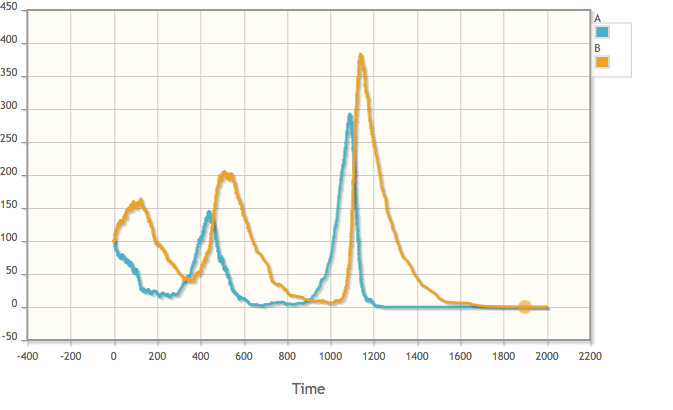
\includegraphics[width=0.53\textwidth]{LVstoch}
\end{center}
  \caption{ODE and stochastic simulation of Lotka Volterra prey-predator model.}\label{LVsim}
\end{figure}



      The \emph{discrete} or \emph{Petri Net semantics} defines a similar transition relation $\lra_D$
over discrete states, but ignoring the rate functions.
      It is thus a trivial abstraction of the stochastic semantics by a forgetful functor, we have
      $$\forall (R_i, M_i, P_i, f_i), {\vec x}\lra_D{\vec x'}\text{ if }      {\vec x}\geq R_i, {\vec x'} = {\vec x} - R_i + P_i$$

The \emph{Boolean semantics} is similar to the discrete semantics
but on Boolean vectors $x$ of $\mathbb{B}^s$,
obtained by the ``zero, non-zero'' abstraction of integers $(>0:\mathbb N\rightarrow\mathbb B$.
With this abstraction, when the number of a molecule is decremented,
it can still remain present, or become absent. It is thus necessary to take into account all the possible
complete consumption or not of the reactants in order to obtain a correct Boolean abstraction
of the discrete and stochastic semantics \cite{FS08tcs}. The \emph{Boolean transition system} $\lra_B$
is thus defined by considering all subsets of the set of reactants $\Set(R_i)$:\\

\noindent
$\forall (R_i, M_i, P_i, f_i), \forall C\in{\cal P}(\Set(R_i)), {\vec       x}\lra_B{\vec x'}$
if ${\vec x}\supseteq \Set(R_i), {\vec x'} =       {\vec x} \setminus C \cup \Set(P_i)$\\


Intgerestingly, with these definitions, the last three semantics are
related by successive Galois connections \cite{FS08tcs}.
The set of Boolean traces is thus a correct abstraction of the stochastic traces for any rate functions,
in the sense that the Boolean abstraction of the stochastic traces is contained in the set of traces of the Boolean semantics.
This means that \emph{if a behaviour is not possible in the Boolean semantics,
  it is not possible in the stochastic semantics} whatever the reaction rate functions are,
and justifies the use of Boolean reasoning tools for many questions.

On the other hand, the differential semantics does not constitute an abstraction of the stochastic semantics,
but provides, under strong assumptions,
 an approximation of the mean stochastic behavior, for instance when the number of each molecule tends to the infinity~\cite{Gillespie77jpc}.
%In the preceding example this condition is obviously not satisfied.


\begin{example}\label{LVbool}
  In the Lotka-Volterra example, one can show that the extinction of the predator is almost sure in the stochastic semantics,
  whereas the differential semantics exhibits sustained oscillations
  (the condition on large numbers of molecules is clearly not satisfied).
  The Boolean semantics exhibits a set of possible Boolean behaviors
  which over-approximates the set of stochastic traces.
   Under this Boolean interpretation, one can observe either
   the stable existence of the prey (in case of extinction of the predator),
   the unstable existence of the predator (which can always disappear),
   or the disappearance of both of them,
but not the extinction of the prey without the preceding extinction of the predator,
nor any Boolean oscillation in absence here of synthesis reaction (e.g.~migration).
These properties can be directly expressed by Temporal Logic formulae described in Section \ref{CTL},
and automatically generated by the model-checking techniques described in Section \ref{MC} as follows:
     \begin{lstlisting}
biocham: present({A,B}).
biocham: generate_ctl_not.
reachable(stable(A))
reachable(steady(B))
reachable(stable(not A))
reachable(stable(not B))
checkpoint(B,not(A))
   \end{lstlisting}
\end{example}

\begin{exercise}\label{LVrExo} Using Biocham v4,
  \begin{enumerate}
  \item Add immigration and emigration reactions for the prey
  \item Compare the different semantics
  \item Explain the relationship between the ODE simulation and the stochastic simulations
    \end{enumerate}
\end{exercise}


In presence of synthesis reactions such as protein synthesis,
the discrepancies between the differential and stochastic interpretations may be less extreme.
For these reasons the differential semantics is widely used for quantitative biological modelling.
The following example shows a typical case of biochemical reaction system for signalling, where the differential semantics approximates the mean stochastic behavior.

\begin{example}\label{MAPK}
  The MAPK (Mitogen Activated Protein Kinase) biochemical reaction system is an extremely frequent signalling module
  that exists in several copies in eukaryote cells for different signalling tasks.
  This network is composed of three stages for a total of 30 reactions, where at each stage a protein gets phosphorylated once or twice, and under this phosphorylated form,
  catalyzes the phosphorylations of the next stage. The input {\small\verb|E1|} of this signalling cascade, directly linked to the transmembrane receptor,
  phophorylates the kinase {\small\verb|KKK|} of the first stage which then phosphorylates the kinase {\small\verb|KK|} which itself phosphorylates the protein {\small\verb|K|}
  to produce the output of the cascade {\small\verb|PP_K|} which can migrate to the nucleus and modify gene transcription.
  Figure \ref{MAPKfig} shows the three levels structure of the reaction system.

\begin{figure}[htb]
\begin{center}
\includegraphics[width=0.7\linewidth]{MAPKgraph} %\includegraphics[width=0.45\linewidth]{MAPKode}
\end{center}
  \caption{MAPK signalling reaction network structure, with three levels of simple (at the first stage) and double (at the second and third stages) phosphorylations, with reverse dephosphorylation reactions catalyzed by phosphatases \cite{HF96pnas}.}\label{MAPKfig}
\end{figure}
\begin{figure}[htb]
\begin{center}
\includegraphics[width=0.5\linewidth]{MAPKode}\includegraphics[width=0.5\linewidth]{MAPKdose}
\end{center}
\caption{ODE simulation of the MAPK signalling model, and dose-response diagram showing stiffer all-or-nothing response at lower levels of the cascade,
  revealing the analog-digital converter function of the MAPK circuit.}\label{MAPKode}
\end{figure}

  Figure \ref{MAPKode} shows the ODE simulation
  and the dose-response diagram (i.e.~{\small\verb|PP_K|}, {\small\verb|PP_KK|} and {\small\verb|P_K|} at steady state versus \verb|E1| varying in the range $[1e-6,1e-4]$).
    This shows that MAPK acts as an analog-digital converter in the cell, with the stiffest response at the third level output \cite{HF96pnas}.
    
\end{example}


\begin{exercise} Using Biocham v4,
  \begin{enumerate}
  \item Load the MAPK model number 9 in BioModels.
  \item Run the commands for drawing the plots in Fig~\ref{MAPKode}.
  \item Search conservation laws.
  \item Simplify the model by using one phosphorylation step only per level, and compare the results.
    \item Keep two phosphorylation steps but simplify the model by using Michaelis-Menten reactions instead of elementary complexation reactions, and compare the results.
    \end{enumerate}
\end{exercise}


It is worth noticing that the reaction inhibitors have not been used for the definition of the hierarchy of semantics in this section.
The reason is that in the differential semantics an inhibitor decreases the rate of a reaction without preventing it completely from proceeding.
One can also define a \emph{Boolean semantics with negation}
where the inhibitors of a reaction are seen as a conjunction of negative conditions that must be satisfied for the reaction to proceed,
by:\\
$\forall (R_i, M_i, P_i, f_i) \forall C\in{\cal P}(\Set(R_i)) {\vec       x}\lra_{BN}{\vec x'}$

\hfill if ${\vec x}\supseteq \Set(R_i), {\vec x}\cap M_i=\emptyset, {\vec x'} =       {\vec x} \setminus C \cup \Set(P_i)$\\
This interpretation is used in many systems, including Boolean Petri Nets
and Rewriting Logic \cite{EKLLMS02psb} yet with no connection to the other semantics.
%This strict interpretation of inhibitors by negations restricts the set of possible Boolean transitions.
%Negative conditions testing the absence of molecules can be added similarly to the Petri Net and stochastic semantics
%but the compatibility with the differential semantics is then lost.

\subsubsection{Hybrid Models}

In the perspective of applying engineering methods to
the analysis and control of biological systems, the issue of building complex models
by composition of elementary models is a central one.
Reaction systems can be formally composed by the multiset union of the reactions
and interpreted in one common semantics,
but there is also a need to compose models with different semantics.
For instance, it makes a lot of sense to combine 
a differential model of protein activation for high numbers of molecules,
with a Boolean or stochastic model of gene expression,
since genes are in single or double copies in a cell. %there is only one copy of a gene in a cell). %~\cite{Pahle09bbi}.

The hierarchy of semantics of reaction systems provides a clear picture for studying the combination of several reaction models with different semantics
and designing hybrid discrete/continuous digital/analog models of cell processes.
A \emph{hybrid model}
is a model obtained by composition of models with heterogeneous semantics
(continuous, stochastic, Boolean, etc.),
and \emph{hybrid simulation} is the topic of simulating such hybrid models.
In \cite{CFJS15tomacs}, it is shown that the combination of events with kinetic reactions,
as already present in SBML, provides  enough expressive power for
combining the discrete and continuous semantics of reaction systems.
Such hybrid reaction systems can also be visualized
as hybrid automata~\cite{Henzinger96lics} in which there is a
state with a particular ODE for each combination of the trigger
values, and there is a transition from one state to another state
when at least one trigger changes value from false to true in the
source state.

Hybrid modelling is used in Systems Biology for reducing the
complexity of modelling tasks \cite{ABIKMPRS01hscc,BZNN13pcb},
e.g.~in signalling 
\cite{GT01hscc}
cell cycle control \cite{SSJT11plos},
gene regulation \cite{MDNM00psb,ABCLR06complexus},
%for speeding up stochastic
%simulations~\cite{HL07jcp,HMMW10cmsb},
and most notably, for achieving whole cell simulation \cite{Karr12cell}.


\subsection{Influence Systems}

Influence systems are a somewhat simpler formalism which is also widely used by modellers
to merely describe the positive and negative influences between molecular species,
without fixing their implementation by biochemical reactions.
In particular, Thomas's regulatory networks form a particular class of Boolean influence systems,
implemented in modelling tools such as GINsim~\cite{NBFLTC09bs}, GNA~\cite{BBCdJDGMMPRR12} or Griffin~\cite{RMCA14alcob}.
It is also worth mentioning that influence systems with spatial information are developed in~\cite{Chazelle12cacm}
as a formalism particularly suitable for describing natural algorithms
in life sciences and social dynamics.
%For these reasons, we present this formalism in parallel to reaction systems.


\subsubsection{Syntax}

In Thomas's framework, a regulatory network is defined by an influence graph given with a Boolean update function for each node.
In order to define the other interpretations of an influence system, we shall distinguish here in the syntax
the conjunctive conditions from the disjunctive conditions,
with the convention that an influence on a target with several sources denotes a conjunctive condition,
while different influences on a same target express a disjunction of conditions. % \cite{FMRS16cmsb}.
%These syntactical conventions are %similar to the formalism of process hitting \cite{PH} and
%a particular case of the concept of multiplexes introduced in \cite{BCK08esm} restricted here to disjunctive normal forms.
%\begin{definition}
   Given a set $S = \{x_1,\dots,x_s\}$ of molecular species, an \emph{influence system}
   $I$ is a set of quintuples $(P, N, t, \sigma, f)$ called \emph{influences}, 
   where $P\subset S$ is called the \emph{positive sources} of the influence, $N\subset S$ the \emph{negative sources}, $t\in S$ is the \emph{target}, 
   \emph{sign} $\sigma\in\{+,-\}$ is the sign of the influence, and $f$ is a real-valued mathematical function
   of $\mathbb{R}^s$, called the \emph{force} of the influence.
%\end{definition}
The influences of sign $+$ are called \emph{positive influences} and those of
sign $-$, \emph{negative influences}. They are noted in Biocham syntax ({\small\verb|f for R/M -> P|}) and ({\small\verb|f for R/M -< P|}) respectively.

\begin{example}\label{LVi}
   The prey-predator model of Lotka--Volterra of Example \ref{LVr} can also be presented by the following system of four influences %between the prey $A$ and the predator $B$:
%   $(\{A, B\}, \emptyset, A, -, k1*A*B)$, $(\{A, B\}, \emptyset, B, +, k1*A*B)$, $(\{A\}, \emptyset, A, +, k2*A)$ and $(\{B\}, \emptyset, B, -, k3*B)$, or in Biocham syntax
   \begin{lstlisting}
k1*A*B for A,B -< A.
k1*A*B for A,B -> B.
k2*A for A -> A.
k3*B for B -< B.
   \end{lstlisting}
   The variant where a species {\small\verb|C|} competes with {\small\verb|A|} for nutrients
   gives an example of negative sources in the positive influences for proliferation:
  \begin{lstlisting}
k2*A/(k4+C) for A/C -> A.
k5*C/(k6+A) for C/A -> C.
   \end{lstlisting}
\end{example}

%Similarly to reaction systems, but
%with a particular condition for the target of a negative influence, 
%we say that 
%over molecular species $\{x_1,\dots,x_s\}$
The distinction between the positive and negative sources of an influence (either positive or negative)
is similar to the distinction between the reactants and the inhibitors of a reaction.
An influence $(P, N, t, \sigma, f)$ is \emph{well formed} if the following conditions hold:
\begin{enumerate}
\item $f(x_1,\dots,x_s)$ is a partially differentiable function, non-negative
   on $\mathbb{R}_+^s$;
\item $x_i\in P$ if and only if $\sigma = +$ (resp.\ $-$) and
   ${\partial {f}}/ {\partial x_i}(\vec x)>0$ (resp.\ $<0$) for some value
   $\vec x\in\mathbb{R}_+^s$;
\item $x_i\in N$ if and only if $\sigma = +$ (resp.\ $-$) and
   ${\partial {f}}/ {\partial x_i}(\vec x)<0$ (resp.\ $>0$) for some value
  $\vec x\in\mathbb{R}_+^s$;
  \item $t\in P$ if $\sigma=-$.
\end{enumerate}
%An influence system is well formed if all its influences are well formed.
%\end{definition}

%For the sake of readibility, an influence $(P, N, t, \sigma, f)$ is also noted in Biocham\footnote{\url{http://lifeware.inria.fr/biocham}} v4 syntax,
%$f \for P/N$\lstinline|->|$t$ if $\sigma=+$, $f \for P/N$\lstinline|-<|$t$ if $\sigma=-$.



\subsubsection{Semantics}\label{semI}

Given a set of species $S=\{x_1,\dots,x_s\}$ and an influence system $\cal I$ over $S$, 
the \emph{differential} semantics associates the following ODE system:

\[
   \frac{dx_k}{dt} = \sum_{(P_i, N_i, x_k, +, f_i) \in \cal I}f_i - \sum_{(P_j, N_j, x_k, -, f_j) \in \cal I}f_j
\]
Intuitively, it adds up all the forces of the positive influences on $x_k$ and
subtracts all the forces of the negative influences on $x_k$ in the derivative of
$x_k$ over time.
For instance, in Example \ref{LVi}, one can check that we get the same ODEs as in Example \ref{LVr}. 

It is worth noticing that the negative sources in a well-formed influence
decrease the force of the influence but do not disable it.
Consequently, the \emph{stochastic} semantics of an influence system with forces,
can be defined similarly to reaction systems, by a transition system, noted $\lra_S$, between discrete states, i.e.~vectors $\vec x$ of $\mathbb{N}^s$,
with the condition that the positive sources are present in sufficient number,
without any condition on the negative sources:
%The transition propensity defined by the force.
      $$\forall (P_i, N_i, A_i, \sigma_i, f_i), {\vec x}\lra_S^{f_i}{\vec x'} \text{ with propensity}f_i\text{ if } {\vec x}\geq P_i, {\vec x'} = {\vec x}\  \sigma_i\ A_i$$
Transition probabilities between discrete states are obtained through
normalization of the propensities of all the enabled transitions,
with time of next reaction~\cite{Gillespie77jpc}.
%      In this interpretation, the negative sources are supposed to decrease the influence propensity but do not prevent the influence from proceeding.
%      They are thus ignored here by the stochastic transition conditions.
      As before, the \emph{discrete} (or \emph{Petri Net}) semantics simply ignores the forces:
      $$\forall (P_i, N_i, A_i, \sigma_i, f_i), {\vec x}\lra_D{\vec x'}\text{ if }      {\vec x}\geq P_i, {\vec x'} = {\vec x}\ \sigma_i\ A_i$$
and the \emph{Boolean semantics} is defined on Boolean vectors $x$ of $\mathbb{B}^s$,
by the ``zero, non-zero'' abstraction.
It is worth noticing that unlike reaction systems, the Boolean semantics associates one transition with one influence,
with the same conditions on Boolean vectors:
$$\forall (P_i, N_i, A_i, \sigma_i, f_i), {\vec       x}\lra_B{\vec x'}\text{
if }{\vec x}\geq P_i, {\vec x'} =       {\vec x}\ \sigma_i\ A_i$$
That Boolean semantics is positive in the sense that it ignores the negative sources of an influence
and contains no negation in the influence enabling condition.

\begin{exercise}\label{LViExo} Using Biocham v4,
  \begin{enumerate}
  \item Compare the different semantics.
    \item Compare the results to the modelling by reactions in Exercise \ref{LVrExo}.
  \item Add immigration and emigration influences and compare the results.
    \end{enumerate}
\end{exercise}

In Lotka-Volterra Examples \ref{LVr} and \ref{LVi},
the Boolean transitions are the same
in this particular case, since there is no reaction that can produce a simultaneous change of the Boolean values of both the prey and the predator.
However in general, reaction systems can produce simultaneous Boolean updates which cannot be represented by an influence system.



\subsubsection{Expressive Power Compared to Reaction Systems}


One can show that any (well-formed) influence system with forces can be represented by a (well-formed) reaction system,
with the same Boolean, discrete, stochastic and differential semantics~\cite{FMRS16cmsb},
i.e.~an influence system can always be simulated by a reaction system for the different semantics.
The converse does not hold for the discrete semantics. For instance for the Boolean semantics, the decomplexation reaction $C$\lstinline|=>|$A+B$,
  has a transition from the state $(A,B,C)=(0,0,1)$ to $(1,1,0)$ which is obviously
  not possible in any influence system since only one variable can change in one transition.
  What is possible is to simulate a reaction system by an influence system which over-approximates its Boolean semantics.

  However, the converse holds for the differential semantics,
  i.e.~(well-formed) influence and reaction systems have the same expressive power~\cite{FMRS16cmsb}.
This means that as far as the differential semantics is concerned,
the influence systems have the same expressive power as reaction systems
and there is no theoretical reason to develop a reaction model.
This does not mean that there is a canonical reaction system associated with an influence system.
Generally, different implementations with reactions are possible without changing the differential semantics.
They represent extra information that is irrelevant to the analysis or simulation of the differential equations,
but can lead to different stochastic simulations for instance.



\subsubsection{Boolean Semantics with Negation \emph{\`a la} Thomas}\label{Thomas}

The formalism of Ren\'e Thomas \cite{TA90book} 
is a Boolean variant of influence systems
which considers negative conditions and deterministic functional updates instead of relational updates.
The success of this formalism lies, on the one hand,
  in the beautiful theory
  of necessary conditions for oscillations and multistability \cite{RRT08aam,Ruet16mfcs} which explains for instance cell differentiation
  by the purely qualitative existence of a positive circuit in the influence graph of the system, and, on the other hand, 
  for its widespread use for the logical modelling of a variety of cell processes beyond gene networks, such as 
  cell cycle \cite{FNLCCT09mb} cell signalling \cite{GCBRKT13plos} or morphogenesis \cite{GCT08bi,SCT08ijdb}.

In the \emph{Boolean semantics with negation},
the negative sources are interpreted as negations in the enabling condition, as follows:
%Formally, the \emph{Boolean with negation semantics} of an influence system is defined by the following transition system:
$$\forall (P_i, N_i, A_i, \sigma_i, f_i), {\vec       x}\lra_{BN}{\vec x'}\text{if }{\vec x}\geq P_i,\ {\vec x}\cap N_i=\emptyset,\ {\vec x'} =       {\vec x}\ \sigma_i\ A_i$$
This interpretation makes it possible to represent any \emph{Boolean unitary transition system}, i.e.~any transition system that updates at most one variable of $\vec x$ in each transition~\cite{FMRS16cmsb}.
%In this case, the state transition graph forms a hypercube.
Furthermore, the Boolean semantics of Thomas's networks is \emph{functional}, in the sense that
the next Boolean state ${\vec x}'$ is defined by a Boolean function $\phi(\vec x)$.
The synchronous semantics is thus deterministic and the non-deterministic asynchronous semantics
is obtained by interleaving, i.e.~by considering all the possible transitions that change the Boolean value of one of the genes at a time.

For these reasons,
a truly non-deterministic influence system such as
$$\{(A,\emptyset,B,+,f),\ (A,\emptyset, B,-,g)\}$$
(for which the transition relation is not a function)
cannot be represented in Thomas's setting.
This excludes self-loops in the state transition graph (on non-terminal states).
This is even more striking in Thomas's multilevel setting, where the above
system can (in the discrete semantics) have transitions from $(1,1)$ both to
$(1,0)$ and to $(1,2)$. That would necessitate the corresponding logical
parameter for $B$ to be at the same time $<1$ and $>1$.
Conversely, any Thomas's gene regulatory network can be represented by an influence system with the Boolean semantics with negation.

  
%\subsection{Horn Clause Representations }\label{prolog}

%\subsubsection{Horn Clause Representation of Reaction Systems ?}

\subsection{Logic Programming}

The transition systems defined in Section \ref{semI} can be straightforwardly represented by Logic Programs (LP), and Constraint Logic Programs (CLP) for the quantitative semantics,
where the states and the transition relation are defined by atoms, and the transition enabling conditions are defined by Horn clauses.
This LP representation of reaction and influence systems suggests the use of a variety of LP tools for reasoning about them,
such as deductive model-checking \cite{DP01sttt,CF03cmsb}, inductive logic programming \cite{Muggleton95ngc,FS08pilp}, probabilistic logic programming \cite{AM02etai} etc.

In \cite{Inoue11ijcai}, it is shown how Thomas's Boolean networks can be directly represented by Normal Logic Programs (NLP),
and how their trajectories and attractors can be computed with methods based on
the similarity between the fixed points of Boolean networks and the immediate consequence operator $T_P$ operator of NLPs.
In particular, point attractors of both synchronous and asynchronous Boolean networks are characterized as the supported models of their associated logic programs so that SAT techniques can be applied to compute them.

Furthermore, NLPs provide a first-order representation which can be used to 
to describe the dynamics of influence systems on an infinite domains, such as the Petri Net semantics.
In return for Logic Programming, this shows that
logic programs that have cyclic attractors and are inconsistent under the supported or stable model semantics \cite{Fages94mlcs}
can have meanings under the ``attractor semantics'' for NLPs.



\section{Automated Reasoning on Model Structures}\label{graph}

%\hfill\emph{``Simplification is the ultimate sophistication'', Leonardo da Vinci.}\\

\subsection{Petri Net Invariants}\label{PN}

Beyond being a useful interpretation of reaction and influence systems in its own right,
the Petri Net semantics provides interesting information on the differential and stochastic semantics of reaction systems.
Petri nets have been introduced historically as a simple chemically-inspired formalism
for describing and analyzing concurrent, asynchronous,
non-deterministic, and possibly distributed, information processing systems \cite{Peterson81book}.
The use of Petri nets for studying biochemical reaction systems, 
by mapping molecular species to places and reactions to transitions,
was considered quite late in~\cite{RML93ismb} for the analysis of metabolic networks.
In this context, the traditional Petri net concepts of place-invariants (P-invariants), transition-invariants (T-invariants),
siphons and traps have shown to have important applications.
This motivated the search for efficient algorithms to scale-up to the size of biological models in model repositories,
and revealed the astonishing performance of SAT and Constraint Logic Programming solvers
which can outperform dedicated algorithms through a straigthforward Boolean or Finite Domain constraint modelling \cite{Soliman12amb,NMFS16constraints}.

A P-invariant is a multiset of places $V$ (i.e.~molecular species) such that the sum of the markings (i.e.~numbers of molecules) remains constant
for any scheduling of the transitions,
i.e.~$V.I=0$ where $I$ 
is the incidence matrix of the Petri net $I=\sum_i P_i-R_i$ with the notations of Section \ref{semR}, i.e.~$I_{ij}$ is the number of arcs from transition $i$ to place $j$, minus the number of arcs from place $j$ to transition $i$.
Such a P-invariant represents a structural conservation law between molecular species,
and corresponds to a linear invariant in the ODE semantics of the reactions,
i.e.~a multiset of differential functions having their sum equal to zero which corresponds to a multiset of molecules whose sum of concentrations remains constant.

\begin{example}\label{MM}
  The Michaelis-Menten enzymatic reaction system is composed of three reactions:
  one of complexation and one of decomplexation of the enzyme with the substrate,
  and one of transformation of the product with release of the enzyme.
  This simple system shown in Figure \ref{MMfig} has two minimal P-invariants which express the conservation of the enzyme in free and complexed form,
  and the conservation of the substrate in free, complexed and product form.
  These structural conservation laws can also be seen in the ODE semantics of the model by summing the corresponding differential functions.
\end{example}

\begin{center}
  \begin{figure}[htb]
  \noindent
  \begin{minipage}{0.5\textwidth}
  \includegraphics[width=5cm]{DAM_mm-crop.pdf}
  \end{minipage}
  \begin{minipage}{0.5\textwidth}
\begin{lstlisting}
E+S => ES.
ES => E+S.
ES => E+P.

biocham: search_conservations.
E+ES
ES+P+S

biocham: list_ode.
d(P)/dt=ES
d(E)/dt=2*ES-E*S
d(ES)/dt=E*S-2*ES
d(S)/dt=ES-E*S
\end{lstlisting}
\end{minipage}
  \caption{Michaelis-Menten system of three reactions representing the binding of an enzyme on its substrate and its transformation in a product,
    and computation of the two minimal P-invariants $\{E,\ ES\}$ and $\{ES,\ P,\ S\}$ corresponding to linear invariants of the differential semantics.
  }\label{MMfig}
  \end{figure}
\end{center}  

  The MAPK model of Example \ref{MAPK} uses Michaelis-Menten reactions for each phophorylation and dephosphorylation step.
  It has seven P-invariants,
  one for each kinase and phosphatase expressing its conservation among its different phosphorylated and complexed forms.

  P-invariants can be computed either by standard Fourier-Motzkin elimination \cite{CS90apn},
or by linear algebra methods such as QR-factorization, Mixed Integer Programming,
or more simply, and in fact more efficiently, by Constraint Logic Programming methods over finite domains, CLP(FD).
The idea here is to solve the equation $V.I=0$ in $V\in\mathbb N^s$ as a Constraint Satisfaction Problem (CSP)
over finite domains by posting
\begin{itemize}
  \item $V.R_i=V.P_i$ for each reaction $i$,
  \item $V.1>0$,
\end{itemize}
and by enumerating the values of $V$ from low to high 
for finding P-invariants that are then checked for minimality by subsumption check  \cite{Soliman12amb}.

Beyond its efficiency, the beauty of the CSP approach is that it generalizes straightforwardly to the computation of other invariants.
T-invariants are the dual notion of P-invariants.
A T-invariant is a multiset $V$ of transitions such that $I.V=0$, i.e.~a multiset of reaction firing that leave invariant any marking.
T-invariants revealed to be equivalent to the notion of extremal fluxes in metabolic networks \cite{KS06bi,ZS03insilicobio,VP94nb},
one of the main tools for analyzing and optimizing metabolic networks \cite{RFBPPWSBP11bi,LB09dam,FSKF09bi,Herrgard08nbt}.
Furhtermore in CSP, just by replacing equality constraints by inequalities, for instance $V.I\le 0$ or $I.V\ge 0$, one can compute 
static subinvariants of markings or fluxes which can only grow or decrease during simulation \cite{Soliman12amb}.
To reduce the combinatorial complexity,
recent results using SAT modulo theory (SMT) solver have shown further improvments for the enumeration of extremal flux modes \cite{PMS14cmsb}.


%Deadlocks and traps in Petri nets as Horn-satisfiability solutions and some related polynomially solvable problems \cite{MB90dam}

Siphons and traps are other interesting Petri Net concepts.
They denote meaningful pools of places that display a specific
behaviour in the Petri net dynamics, and that guarantee some persistence properties, independently of the rate functions.
A siphon is a set of places that, once unmarked, remains unmarked. A trap is a
set of places that, once marked, can never loose all its tokens.
These structural properties provide sufficient conditions 
for reachability (whether the system can produce a given protein or reach a given state from a given initial state) and liveness 
(deadlock freedom from a given initial state) properties in ordinary Petri nets.
%It is proved that in order for a net to have all its transitions live, it is necessary that each siphon remains
%marked. One way to keep each siphon marked is to
%have a marked trap inside it. In fact, this condition is necessary and
%sufficient for a free-choice net to be live~\cite{Peterson81book},
It has been shown %in~\cite{TYW96ieice} and~\cite{YW99eice}
that the problems of existence of a minimal siphon
of a given cardinality, or containing a given place, are NP-complete. 
In \cite{NMFS16constraints}, 
a Boolean model is proposed to solve these minimal enumeration problems,
either by calling a SAT solver iteratively,
or by backtracking with a Constraint Logic Program (CLP)
over Booleans.
Interestingly, the SAT and CLP solvers both outperfom by one or two orders of magnitude
the state-of-the-art algorithms from the Petri net community described in~\cite{CFP05ieee} 
for computing minimal sets of siphons and traps,
that have already been shown to outperform
Mixed Integer Linear Programs. % previously proposed in~\cite{Murata89ieee,CFP02ieee}.
On a benchmark of 345 biological models from the curated part of the BioModels repository~\cite{NBBCDDLSSSSH06nar},
the Boolean method for enumerating the set of all minimal siphons
takes a few seconds in MiniSAT. It also scales very well in the size of the net.
%and to the number of minimal siphons which remains however relatively small in these instances.
The CLP(B) program also solves all but one instances of the benchmark,
with a better performance than MiniSAT in average, but does not scale-up as well on the largest size
Petri nets, such as for instance on Kohn's map with 509 species and 775 reactions.
The efficiency of the MiniSAT and CLP(B) methods 
for enumerating in a few seconds the set of all solutions of an NP-complete problem for
all, including large, instances of the BioModels benchmark
is quite surprising.
In \cite{NMFS16constraints}, it is shown that the SAT phase transition threshold and complexity wall is traversed on those instances,
but that the problem is tractable on graphs with bounded treewidth % (by Courcelle's theorem on monadic second§order logic  \cite{Courcelle90ic})
which seems to be the case of biochemical networks since most models in BioModels have a small treewidth less than 10.
Still this does not explain why SAT and CLP solvers perform so well on this problem.


\subsection{Model Reductions by Graph Matching}\label{reduc}

Models in Systems Biology are built with two somewhat contradictory perspectives:
\begin{itemize}
\item Models for aggregating knowledge on particular cell processes, in this perspective the more detailed the better;
\item Models for answering particular questions on cell processes, in this perspective the more abstract the better,
  for getting rid of useless details that are not necessary to the questions at hand.
\end{itemize}
One way to reconcile these two perspectives is to relate models by model reduction relationships,
that is currently not the case in model repositories.
Model reduction is a central topic in dynamical systems theory, for reducing the complexity of detailed models,
finding important parameters, and developing multi-scale models for instance.
While perturbation theory is a standard mathematical tool to analyze the different time scales of a dynamical system,
and decompose the system accordingly, Systems Biology needs novel methods for comparing and reducing models on a very large scale.

Graph matching techniques can be used to detect model reduction relationships between models within large repositories like BioModels.
However the standard notion of subgraph isomorphism (SISO) for finding graph motifs is not adequate.
For instance, the very basic reduction of Michaelis Menten which consists in reducing the system of three reactions of Example \ref{MM}
to one single catalytic reaction {\small\verb|E+S => E+P|},
produces the graph
\begin{center}
  \includegraphics[width=0.25\linewidth]{DAM_mmr-crop.pdf}
  \end{center}
which is not isomorphic to a subgraph of the graph of Example \ref{MM}.
%shown in Figure \ref{MMred} which are not comparable by subgraph isomorphism.
%
%\begin{figure}[htb]
%\hfill\includegraphics[width=0.5\linewidth]{DAM_mm-crop.pdf}\hfill\includegraphics[width=0.3\linewidth]{DAM_mmr-crop.pdf}\hfill
%\caption{Bipartite graphs representing respectively the Michaelis-Menten system of 3 reactions and its reduction to one catalytic reaction.}\label{MMred}
%\end{figure}
In this example, the reduced graph can be obtained from the source graph by a sequence of \emph{delete and merge operations on species and reaction} vertices.
These transformations can typically be justified in chemistry by considering for instance: (i) reaction deletions for slow reverse reactions, (ii) reaction mergings for reaction chains with a limiting reaction, (iii) molecular species deletions for species in excess and (iv) molecular mergings for quasi-steady state approximations.

This operational view of graph reduction by graph transformation operations
is equivalent to the existence of a subgraph (corresponding to delete operations) epimorphism (i.e.\ surjective homomorphism, corresponding to merge operations) from a source graph to a reduced graph \cite{GSF10bi}.
Formally, let $G$ and $G'$ denote graphs, with $G = (V, A)$ and $G' = (V', A')$,
  an {\em epimorphism} from $G$ to $G'$ is a surjective function $f: V \rightarrow V'$
  such that
  \begin{itemize}
  \item for all $u, v \in V$, if $(u, v) \in A$, then $(f(u),f(v))\in A'$ (graph homomorphism), and,
  \item for all $(u', v') \in A'$, there exists $(u, v) \in A$ such that $f(u) = u'$ and $f(v) = v'$
    (surjectivity on arcs).
  \end{itemize}
  The {subgraph} of $G$ induced by a subset of vertices $U\subseteq V$ of $G$, is $G_{\downarrow U}=(U,A \cap (U\times U))$.
  A {\em  subgraph epimorphism} (SEPI) from $G$ to $G'$ is an epimorphism $f$ from an induced subgraph $G_0$ of $G$ to $G'$.
%\end{definition}

In Example \ref{MM}, the two graphs of the Michaelis-Menten reduction,
are related by a SEPI where the induced subgraph 
of the first graph is obtained by deleting the vertices $ES$ and $d$,
and where both reaction vertices $c$ and $p$ are mapped to the vertex $c$ of the second graph.

Subgraph epimorphisms differ from subgraph isomorphisms 
by allowing merge operations in addition to delete operations.
On undirected graphs, SEPIs differ from graph minors %\cite{Lovasz06bams}
in several points: non adjacent vertices may be merged,
 merging adjacent vertices creates loops, 
and arcs cannot be deleted without deleting or merging vertices.
Determining whether there exists a SEPI from a graph $G$ to a graph $G'$ is NP-complete \cite{GFMSS14dam}.
Nevertheless a simple CLP(FD) program or SAT solver can solve this problem on all pairs of reaction graphs in the repository BioModels
with just a few timeouts for some pairs of models.
%This program encodes the mathematical definition of SEPI
%with constraints over finite domains and a simple search strategy for enumerating all solutions by backtracking.

Graph morphisms can be modelled by introducing one variable per node of the source graph,
with  the set of  nodes of the target graph as integer domain.
A variable assignment then represents a mapping from the source nodes to the target nodes.
The morphism condition itself is written with  a tabular constraint of CLP(FD) %({\tt fd\_relation} in GNU-Prolog \cite{gprolog}),
which forces a tuple of variables to take its value in a list of tuples of integers.
The surjectivity property can be enforced by creating variables for the target arcs
with the set of source arcs as domain, and using the global constraint
{\tt all\_different} of CLP(FD).
Then, the enumeration on the target arc variables
enforces surjectivity and  the enumeration of node variables enforce the
computation of a complete morphism \cite{GFMSS14dam}.

\begin{figure}[htb]
\begin{center}
\includegraphics[width=\linewidth]{sepi-mapk.png}
\end{center}
\caption{Hierarchy of MAPK models in BioModels automatically constructed by SEPI matching.
Schoeberl's model 14 and Levchenko's model 19 are not represented here,
they do not map each other but map to the other models.}
\label{fig:mapk}
\end{figure}

Figure~\ref{fig:mapk} shows the hierarchy of MAPK signalling models
in BioModels that has been automatically reconstructed by graph matching, i.e.~by computing SEPIs between all pairs of models.
The arrows between models denote model reductions and double arrows denote reaction graph isomorphisms,
e.g.~between models 9 and 11 which differ just by molecule names and rate functions.
These models have the same structure shown in Example \ref{MAPK}.
They reduce to model 10 which is also three level but without the reverse dephosphorylation reactions.
It reduces also to models 29 and 27 which are one level models with ad without the dephosphorylation reactions.


\section{Modelling Dynamical Behaviours}\label{temporal}


\subsection{Propositional Temporal Logics}\label{CTL}

In the early days of computational Systems Biology, propositional temporal logic
was soon proposed by computer scientists to formalize the Boolean properties of the behaviour of
biochemical reaction systems 
\cite{EKLLMS02psb,CF03cmsb} and gene influence systems \cite{BCRG04jtb,BRdJ05bi}.
In this approach, it is possible to
evaluate qualitatively, at a high level of abstraction, what may or must  happen in interaction networks of large size (e.g.~of one thousand reactions and species),
and also to compute the initial conditions that exhibit a particular behaviours.
This can be achieved by using the powerful symbolic model-checking tools
designed over the last decades for circuit and program verification \cite{CGP99mit,CCGGPRST02cav}
using SAT solvers.

The {\em Computation Tree Logic} CTL$^*$ \cite{CGP99mit}
is an extension of
classical logic which allows reasoning on an infinite tree of Boolean state transitions from an initial state.
It uses modal operators about branches (non-deterministic choices) and time (state
transitions) to qualify where and when a proposition is true. Two path quantifiers $A$ and $E$ are thus introduced to handle
non-determinism: $A\phi$ meaning that $\phi$ is true on all paths,
and $E\phi$ that it is true on at least one path.
Several time operators are introduced,
$X\phi$ means that $\phi$ is true
 at the next state,
$G\phi$ (globally) that $\phi$ is true in all future states,
$F\phi$ (finally) that $\phi$ is true in some future state,
$\phi \U\psi$ (until) that $\phi$ is always true before $\psi$ becomes true,
and $\phi\R\psi$ (release) that $\psi$ is either globally true or always true up to the first occurrence of $\psi$ included.
Table \ref{CTLtruth} defines the truth value of a formula in a Kripke
structure where the states are defined by Boolean variables. 
In this logic, $F\phi$ is equivalent to $\true \U \phi$, 
$G\phi$ to $\phi\R \false$, 
and we have the following duality properties:
$\neg\X\phi=\X\neg\phi$,
$\neg\E\phi=\A\neg\phi$, 
$\neg\F\phi=\G\neg\phi$, 
$\neg(\phi \U \psi) = \neg\phi \R \neg\psi$.

\begin{table}[htb]
\begin{center}
\begin{tabular}{|lll|}
\hline
 $s\models\alpha$ & if &  $\alpha$ is a propositional formula true in the
 state $s$,\\
 $s\models E\phi$ & if &  there exists a path $\pi$ starting from $s$ s.t. $\pi\models\phi$,\\
 $s\models A\phi$ & if &  for all paths $\pi$ starting from $s$, $\pi\models\phi$,\\
 $\pi\models \neg\phi$ & if &  $\pi\not\models\phi$, \\
$\pi\models\phi\ \wedge\ \psi$ & if &  $\pi\models\phi$ and  $\pi\models\psi$, \\
$\pi\models\phi\ \vee\ \psi$ & if &  $\pi\models\phi$ or  $\pi\models\psi$, \\
 $\pi\models\phi\Rightarrow\psi$ & if &  $\pi\models\neg\phi$ or $\pi\models\psi$, \\
 $\pi\models\phi$ & if &  $s\models\phi$ where $s$ is the first state of $\pi$, \\
 $\pi\models \X\phi$ & if &  $\pi^1\models\phi$, \\
 $\pi\models \F\phi$ & if &  $\exists k\ge 0$ s.t. $\pi^k\models\phi$, \\
 $\pi\models \G\phi$ & if &  $\forall k\ge 0$, $\pi^k\models\phi$, \\
 $\pi\models \phi \U \psi$ & if & $\exists k\ge 0$ s.t.
$\pi^k\models\psi$ and $\pi^j\models \phi$ $\forall j\ 0\le j<k$.\\
 $\pi\models \phi \R \psi$ & if & $\forall k\ge 0$ $\pi^k\models\psi$ or $\exists j<k\ \pi^j\models \phi$\\
\hline
\end{tabular}
\end{center}
\caption{Inductive definition of the truth value of a CTL$^*$ formula in a given
state $s$ or path $\pi$, for a Kripke structure $K$.}
\label{CTLtruth}
\end{table}

The LTL fragment of CTL$^*$ contains no path quantifier. An LTL formula is true if it is true on all paths.
The CTL fragment of CTL$^*$
enforces that each temporal operator is preceded
by a path operator, and each path operator is immediately followed by a
temporal operator.
In the context of computational Systems Biology,
the following abbreviations for CTL formulae are particularly useful to analyze Boolean attractors \cite{CF03cmsb,TFFT16bi}: %,CCDFS04tcs,FSC04jbpc,CFS04cmsb},
\begin{itemize}
   \item {\small\tt reachable(P)} stands for $\EF(P)$;
   \item {\small\tt steady(P)} stands for $\EG(P)$;
   \item {\small\tt stable(P)} stands for $\AG(P)$;
   \item {\small\tt      checkpoint(Q,P)} stands for $\neg E(\neg Q \U P)$;
   \item {\small\tt oscil(P)} stands for $\AG ((\EF\ P) \wedge (\EF\ \neg P))$.
%   \item {\small\tt loop(P,Q)} stands for $\AG ((P \Rightarrow \EF\ Q) \wedge (Q \Rightarrow \EF\ P))$.
\end{itemize}
It is worth noting that that notion of checkpoint here is correlational but not necessarily causal.
The last abbreviation is actually a necessary but not sufficient condition for oscillations.
The correct formula for oscillations is indeed the CTL$^*$ formula
$\EG (\F P\ \wedge \F\neg P)$ which cannot be expressed in CTL.
%Of course such abbreviations can be composed, for instance
%the formula {\small\tt \AG(!P -> checkpoint(Q,P))} expresses that $Q$ is a (correlational) checkpoint for $P$ not only in the initial state
%but in all reachable states.
The formula {\small\tt reachable(stable(P))} which is not expressible in LTL, expresses that the state denoted by formula $P$ is a reachable stable state.
In Example \ref{LVbool}, these formulae are used as patterns to enumerate the interesting properties
of the Boolean semantics of the prey-predator system.



\subsection{Quantitative First-Order Temporal Logics} % Thresholds and Timing Constraints}

Generalizing temporal logic techniques to quantitative models can be done in two ways:
either by discretizing the different regimes of the dynamics in piece-wise linear or affine models \cite{BPCGMJ10bi,BBJGM04iswmcss,JGHPSG04bmb},
or by taking a first-order version of temporal logic  with constraints on concentrations,
as query language for the numerical traces \cite{APUM03cbp,FR08tcs,DM10formats}.
The first approach brings us back to symbolic propositional methods to analyze quantitative models \cite{BBCdJDGMMPRR12}.
In this section, we present the second approach.
%The temporal logic approach to the specification of imprecise dynamical properties of biological systems
%can also be made quantitative and applied to quantitative models over concentrations.

The idea is to lift it to a first-order setting with numerical (linear) constraints over the reals,
in order to express threshold and timing constraints and more complex constraints on the concentrations of the molecular compounds.
For instance, the reachability of a threshold concentration for a molecule $A$
can be expressed with the formula $\F(A>v)$ for some value or free variable $v$.
Such formulae can then be interpreted on a finite numerical trace (extended with a loop on the last state)
obtained either from a biological experiment, 
or from the numerical simulation of an ODE model,
giving the concentrations of the molecules at discrete time points, e.g.~Figure \ref{trace}.


\begin{figure}[htbp]
\centering
\includegraphics[width=0.7\linewidth]{trace.png} %time_series}
\caption{ \label{trace} Numerical trace depicting the time evolution of a protein concentration.}
\end{figure}


\begin{table}[htb]
\it
\begin{center}
\begin{tabular}{ll}
$\phi$ ::=& c \ $|$\  $\phi\Rightarrow\psi$\ $|$\  $\phi\wedge\phi$\ $|$\  $\phi\vee\phi$ 
   $|$\   $\X\phi$\ $|$\   $\F\phi$\ $|$\  $ \G\phi$ 
   $|$\  $\phi\U\phi$ \ $|$\  $\phi\R\phi$\\
\end{tabular}
\end{center}
\caption{Grammar of FO-LTL($\Rlin$) formulae where $c$ denotes linear constraints over molecular concentrations,
free variables and the time variable.}
\label{foltl}
\end{table}

This is possible in the First-Order Linear Time Logic with linear constraints over the reals (FO-LTL($\Rlin$))
and in different variants like Signal Temporal Logic \cite{DM10formats}.
%to specify semi-qualitative semi-quantitative properties of a biological dynamical system.
%LTL is the fragment of CTL$^*$ without any path quantifier and only time operators interpreted on a trace.
Table \ref{foltl} summarizes the grammar of FO-LTL($\Rlin$) formulae.
Timing constraints can be expressed with the time variable and free variables to relate 
the time of differents events.
For instance, the formula $\G(Time\le t_1\Rightarrow[A]<1\wedge Time\ge t_2\Rightarrow[A]>10)\wedge(t_2-t_1<60)$
expresses that the concentration of molecule $A$ is always less than 1 up to some time $t_1$,
always greater than 10 after time $t_2$, and the switching time between $t_1$ and $t_2$ is less than 60 units of time.
A local maximum for molecule concentration $A$ 
can be defined with the formula $\F(A\le x\wedge\X(A=x\wedge\X A\le x))$.
This formula can be used to define oscillation properties, with period constraints
defined as time separation constraints between the local maxima of the molecule,
as well as phase constraints between different molecules \cite{FT14book}.

The {\em validity domain} $\cl{D}_{(s_0,...,s_n), \phi}$
of the free variables of an FO-LTL($\Rlin$) formula $\phi$ on a finite trace $(s_0,...,s_n)$,
can be computed by finite unions and intersections of polyhedra, by a simple extension
of the model-checking algorithm to a constraint solving algorithm \cite{FR08tcs,FR09cp}, as follows:
\begin{itemize}
\item $\cl{D}_{(s_0,...,s_n), \phi} = \cl{D}_{s_0, \phi}$,
\item $\cl{D}_{s_i, c(\vct x)} =\{\vct{v}\in \mathbb{R}^k \mid\ s_i\models c[\vct{v}/\vct{x}] \}$ for a constraint $c(\vct x)$,
\item $\cl{D}_{s_i, \phi\wedge \psi} = \cl{D}_{s_i, \phi} \cap \cl{D}_{s_i, \psi}$,
\item $\cl{D}_{s_i, \phi\vee \psi} = \cl{D}_{s_i, \phi} \cup \cl{D}_{s_i, \psi}$,
\item $\cl{D}_{s_i, \op{X}\phi} = \cl{D}_{s_{i+1}, \phi},$
\item $\cl{D}_{s_i, \op{F}\phi} = \bigcup_{j=i}^n \cl{D}_{s_{j}, \phi}$,
\item $\cl{D}_{s_i, \op{G}\phi} = \bigcap_{j=i}^n \cl{D}_{s_{j}, \phi}$,
\item $\cl{D}_{s_i, \phi\op{U}\psi} = \bigcup_{j=i}^n ( \cl{D}_{s_{j}, \psi} \cap \bigcap_{k=i}^{j-1} \cl{D}_{s_{k}, \phi} )$.
\end{itemize}


For instance, on the numerical trace of Figure \ref{trace},
the validity domain, depicted in Figure \ref{domain},
of the formula $\F(A\ge y_1\wedge\F(A\le y_2))$, where $y_1$ and $y_2$ are free variables,
is $y_1\le 10\wedge y_2\ge 2$.
This can be used for analyzing experimental traces,
and extracting logical formulae from data time series.




\begin{figure}[htb]
\centering
\includegraphics[width=0.7\linewidth]{domain2.png} %time_series}
\caption{ \label{domain} Validity domain of the formula $\F(A\ge y_1\wedge\F(A\le y_2))$
on the trace of Figure \ref{trace}.
The two points correspond to the formulae $\phi_1=\F(A\ge 7\wedge\F(A\le 3))$ (true)
and $\phi_2=\F(A\ge 7\wedge\F(A\le 0))$ (false) respectively.}
\end{figure}


%\subsection{Continuous Satisfaction Degree}\label{sd}

However, for some important applications such as parameter search, sensitivity and robustness measures, presented in Section \ref{sens}
the classical true/false valuation of a logical formula is not well suited.
State-of-the-art continuous optimization algorithms
such as evolutionary algorithms require a fitness function
to measure progress towards satisfiability,
i.e.~they require to valuate TL formulae with a continuous satisfaction degree in the interval $[0,1]$.


\begin{centering}
\begin{figure}[htb]
\centering
\includegraphics[width=0.8\linewidth]{tyson.png}
\caption{Landscape of the continuous satisfaction degree of an oscillation property with amplitude constraint,
on a color scale from yellow to black,
as a function of two parameters in a quantitative model of the yeast cell cycle from \cite{Tyson91pnas}. 
The parameter sets $\vct{k}_A$, $\vct{k}_B$ and $\vct{k}_2^*$
satisfy the specification \cite{RBFS11tcs}. 
The parameter sets $\vct{k}_c$ and $\vct{k}_2$ violate the amplitude constraint.
The non-yellow zone where there are oscillations is equivalently delimited by the bifurcation diagram considered in \cite{Tyson91pnas}. 
%CMA-ES iteratively samples the landscape to find a path in a random walk from $\vct{k}_2$ to $\vct{k}_2^*$ for instance.
}
\label{tyson}
\end{figure}
\end{centering}



A method based on variable abstraction is described in \cite{RBFS09bi,RBFS11tcs} for computing the continuous satisfaction degree 
of an FO-LTL($\Rlin$) formula over a numerical trace.
A closed formula, for instance
$$\phi_2=\F(A\ge 7\wedge\F(A\le 0)),$$
is first abstracted in a formula with free variables by replacing constants with free variables, 
i.e.~$$\phi=\F(A\ge y_1\wedge\F(A\le y_2))$$
with the objective values 7 for $y_1$ and 0 for $y_2$.
Then, the validity domain $\cl{D}_{T, \phi}$ of the formula $\phi$ on a trace $T$
%obtained by simulation for some parameter values,
makes it possible to define the {\em violation degree} $vd(T,\phi,o)$ of the formula on $T$ with objective $o$,
simply as the distance between the validity domain and the objective point $o$, 
e.g.~2 in Figure \ref{domain}.
A {\em continuous satisfaction degree} in the interval $[0,1]$
can then be defined by normalization as the inverse 
of the violation degree $d$ plus one, i.e.~1/3 in Figure \ref{domain}:
$$sd(T,\phi,o)={\frac1{1+vd(T,\phi,o)}}$$

In a model of the yeast cell cycle by Tyson \cite{Tyson91pnas},
a FO-LTL($Rlin$) formula of oscillation with amplitude constraint
produces the landscape of continuous satisfaction degree depicted in Figure \ref{tyson}
obtained by varying two parameters of the model.
Such a landscape is compatible with bifurcation diagrams
but is not limited in dimension and can be used for robustness measures and parameter search as shown in Sections \ref{sens} and \ref{search}.

\section{Automated Reasoning on Model Dynamics}\label{dynamic}

%\hfill\emph{``Art lives from constraints and dies from freedom'', Leonardo da Vinci.}\\

\subsection{Symbolic Model-Checking of Biochemical Circuits}\label{MC}

Regulatory, signalling and metabolic networks are very complex mechanisms which are far from being understood on a global scale.
Data on the rate functions of the individual reactions are also rare and unreliable, 
making the building of quantitative models particularly challenging in many cases.
In those situations, qualitative analyses can however be conducted
in the Boolean semantics of the reactions,
using the powerful model-checking tools developed for circuit and program verification \cite{CGP99mit} in the last decades.


\begin{figure}[htb]
\begin{center}
\includegraphics[width=\linewidth]{Kohn.jpg}
\end{center}
\caption{Kohn's map of the mammalian cell cycle control \cite{Kohn99mbc}.}\label{Kohn}
\end{figure}

Figure \ref{Kohn} reproduces Kohn's map of the mammalian cell cycle \cite{Kohn99mbc}
using some graphical conventions introduced by K. Kohn to represent the different types of interactions
(complexation, binding, phosphorylations, modifications, synthesis, etc.).
This map has been transcribed in a reaction model of 732 reaction rules
over 165 proteins and genes, and 532 variables taking into account the different forms
of the molecular species \cite{CCDFS04tcs}.
The astronomical number of Boolean states in this system, $2^{532}$,
prevents the explicit representation of the state graph,
however, a set of states in this space can be represented \emph{symbolically}
by a Boolean formula over 532 variables,
and the transition relation by a Boolean formula over twice that number of variables.
For instance the formula $\false$ represents the empty set, $\true$ the universe of all states, 
$x$ the set of $2^{531}$ states where $x$ is present, etc.
The results reported in \cite{CCDFS04tcs} showed the performance of the state-of-the-art symbolic model checker NuSMV \cite{CCGGPRST02cav}
using the representation of Boolean formulae by ordered binary decision diagrams (OBDD),
on this non standard transition system from biology.
The compilation of the whole 732 reactions into Boolean formulae took 29 seconds,
and simple reachability and oscillations properties could be checked in a few seconds.
Furthermore in this example, the negative answer to the query concerning the oscillation of cyclin B
revealed the omission of the synthesis of cyclin B in the map.


A symbolic model-checker can also compute the set of initial states, represented by a \emph{boolean constraint}, for which a formula is true.
This  may suggest biological experiments to verify a CTL property predicted by the model,
in particular conditions on the real biological object \cite{BCRG04jtb}.
For instance, the checkpoints proved in a model of the cell cycle, or of a signalling network, 
provide possible drug targets to block the cell cycle or a signalling cascade.


\subsection{Parameter Sensitivity and Robustness Measure}\label{sens} %of an FO-LTL($\Rlin$) Property}

In \cite{Kitano07msb}, Kitano gives a general definition
of the \emph{robustness} of a property $\phi$
in a system with respect to a set $P$ of perturbations given with their probability distribution,
as the mean functionality of the system with respect to $\phi$ under the perturbations.,
%with the system's functionality defined in an {\em ad hoc} way for each property.
In the FO-LTL($\Rlin$) Temporal Logic framework, this definition instanciates straightforwardly
to a computable notion of robustness of a property of a system,
simply by taking the continuous satisfaction degree as functionality measure \cite{RBFS09bi}, i.e.
$$\Rob_{S,\phi,P}=\int_{p\in P} \pprob(p)\; sd(T_p,\phi)\; dp.$$
In a model, this mathematical definition of robustness can be evaluated by 
%\begin{enumerate}
(i) sampling the perturbations according to their distribution,
(ii) measuring the satisfaction degree of the property
for each simulation of the perturbed model,
 and (iii) returning the average satisfaction degree.
%\end{enumerate}

This methodology has been used in \cite{BYWB07bi} to design 
a robust switch satisfying some timing constraints
implemented \emph{in vivo} by synthetic biology means with an artificial cascade of gene inhibitions.
Moreover, continuous parameter \emph{sensitivity indices} computed in this approach
determined the most important parameters for improving the robustness of the design with respect to the timing constraints,
that unexpectedly appeared to be the degradation rate parameters.


On the quantitative model of the yeast cell cycle \cite{Tyson91pnas}
and the oscillation with amplitude constraint depicted in Figure \ref{tyson},
the estimated degree of robustness for parameters $\vct{k}_A$, $\vct{k}_B$ and $\vct{k}_C$
 are respectively 0.991, 0.917 and 0.932. This is consistent with the location 
of points $\vct{k}_A$, $\vct{k}_B$ and $\vct{k}_C$.
Perturbations around point $\vct{k}_A$  have high probabilities of staying in the region satisfying the specification whereas perturbations around point $\vct{k}_B$  have high probabilities of moving the system to the region with no oscillation. $\vct{k}_C$ is more robust than $\vct{k}_B$ even though, as opposed to $\vct{k}_B$, its violation degree is non null. This is explained by the abrupt transition between oscillating and non oscillating regions near $\vct{k}_B$ compared to the smoother
transition near $\vct{k}_C$.



\subsection{Parameter Search}\label{search}


Probably the most central difficulty in quantitative systems biology, is that the kinetic parameter values
of biochemical reactions are usually unknown, but are mandatory for building quantitative models.
They must thus be estimated from
the observation behaviour of the system under various conditions:
gene knock-outs, differences of milieu, drugs,  etc.

This problem amounts to solve the inverse problem
of finding the parameter values of an ODE model for reproducing experimental curves,
or, more appropriately, the relevant properties of the experimental curves.
The formalization of those properties in quantitative temporal logic
is particularly useful in biology where experimental data may be imprecise in nature,
with important cell-to-cell variability, and irregular oscillation periods and phases.
The continuous satisfaction degree of FO-LTL($\Rlin$) formulae 
provide the necessary objective or fitness function to apply black box optimization algorithms
with the all bunch of meta-heuristics \cite{SGH11ieee} such as Particle Swarm Optimization (PSO),
Genetic Algorithms (GA), Neural Networks
and portfolio algorithms for parameter estimation  \cite{Banga08bmc}.

Of particular relevance in this context, is the Covariance Matrix Adaptation Evolution Strategy (CMA-ES) of N. Hansen \cite{HO01ec}
which enjoy all desirable invariance properties
with respect to scaling and symmetries.
CMA-ES can be used with the satisfaction degree of an FO-LTL($\Rlin$) specification as fitness function,
for searching kinetic parameter values, initial concentrations or control parameters \cite{RBFS11tcs}.
On the quantitative model of the cell cycle of \cite{Tyson91pnas},
Figure \ref{tyson} depicts
the landscape of the satisfaction degree of an oscillation property with amplitude constraint,
as a function of two parameters of the model.
This landscape is iteratively sampled by CMA-ES meta-heuristics to find a path towards satisfaction,
and optimize the model parameter values,
for instance going from $\vct{k}_2$ to $\vct{k}_2^*$ in a few steps.


This strategy for optimizing parameters with respect to an FO-LTL($\Rlin$) specification
makes it possible to solve a wide variety of problems in computational systems biology,
for fitting models to experimental data in high dimension, up to 100 parameters.
This methodology has been used in  \cite{HDGRAKVDGPCPCFLR12msb}
to elucidate the complex quantitative dynamics of GPCR cell signalling networks,
by revisiting the structure of the known reactions following the failure of CMA-ES to fit the FO-LTL($\Rlin$) properties of some mutants,
making new biological hypotheses based on sensitivity analyses,
and verifying them by new biological experiments.
In \cite{TFSDF16biosystems}, it served to build  a quantitative model of the cell cycle and the circadian clock
and predict clock gene up-regulation during mitosis in embryonic fibroblasts.

The same strategy for parameter optimization can also be used
to compute control parameters in order to achieve a desired behaviour
at the single cell or cell population levels.
This has been shown for long-term model-based real-time control of
gene expression in yeast cells using a microfluidic device in \cite{UMDCFBBH12},
and in the context of cancer chronotherapies, at the whole body scale, to couple models of the cell cycle, circadian clock, 
DNA repair system and drug metabolism,
to optimize anti-cancer drug administration laws in \cite{BDACOCL11plos,DFRS11tcs}.



\section{Learning Mechanistic Models from Temporal Data}\label{learning}

Biological modelling is still an art which is currently limited in its applications by the number of available modellers.
Automating the process of model building is thus a very desirable goal
to attack new applications, develop patient-tailored therapeutics,
and also design experiments that can now be largely automated
with a gain in both the quantification and the reliability of the observations, at both the single cell and cell population levels.

Machine learning is revolutionarizing the statistical methods in biological data analytics,
data classification and clustering, and for making predictions from static measurements.
However, learning dynamical models from temporal data is more challenging.
There has been early work on the use of machine learning techniques, such as inductive
 logic programming \cite{Muggleton95ngc} combined with active learning in the vision of the ``robot scientist'',
to infer gene functions \cite{BMOKRK01etai},
metabolic pathway descriptions \cite{AM02etai,AM02slps}
or gene influence systems \cite{BCRG04jtb},
or to revise a reaction model with respect to CTL properties \cite{CCFS06tcsb}.
Since a few years, progress in this field can be measured on public benchmarks
of the ``Dream Challenge'' competition \cite{Meyer14bmc}.
In this fastly moving field, we focus here on a general purpose framework for learning the structure of a mechanistic model.

\subsection{Probably Approximatively Correct Learning}\label{pac}

In his seminal paper on a theory of the learnable \cite{Valiant84cacm},
Valiant questioned what can be learned from a computational viewpoint,
and introduced the concept of probably approximate correct (PAC) learning,
together with a general-purpose polynomial-time learning protocol.
Beyond the learning algorithms that one can derive with this methodology,
Valiant's theory of the learnable has profound implications
on the nature of biological and cognitive processes,
of collective and individual behaviors,
and on the study of their evolution \cite{Valiant13book}.
In this section, we simply recall the general theory of PAC learning,
and illustrate it with the learning of Boolean gene networks from gene expression data.

The learning protocol for Boolean functions considers
a finite set of Boolean variables $x_1,\ldots,x_s$.
A vector is an assignment of the $s$ variables to $\{0,1,*\}$
where the symbol $*$ denotes the undetermined.
A vector is total if it contains no undetermined value.
A Boolean function $F:\{0,1\}^s \rightarrow\{0,1\}$
assigns a Boolean value to each total vector.
A Boolean concept $C:\{0,1,*\}^s \rightarrow\{0,1\}$
assigns similarly a Boolean value to non total vectors,
with the following independence constraint:
for any vector $v$ and any total extension $w$ of $v$ (i.e.~where the undetermined values in $v$ are replaced by $0$ or $1$)
we have $C(v)=C(w)$.

The PAC learning protocol considers a hidden Boolean function $F$,
a class $\cal M$ of models to learn, $f(x_1,...,x_s) \in \{0,1,*\}$,
a set of positive examples, i.e.~a set of vectors $v$ for which $F(v)=1$,
and an arbitrary probability distribution $D$ over this set
for representing the relative frequency of the positive examples.
The restriction to positive examples is for the sake of simplicity.
The PAC learning protocol then allows for
\begin{itemize}
  \item
calls for positive examples, i.e.~vectors $v$ such that $F(v)=1$ given with probability $D(v)$,
  \item
calls for oracle on some input $v$ to know the value of $F(v)$
\end{itemize}

\begin{example}
  This Boolean framework perfectly fits the Boolean semantics of Thomas's gene regulatory networks described in Section \ref{Thomas}.
  Indeed in that formalism, each gene $x_1,\ldots,x_s$ is given with a Boolean function  $F_{x_i}:\{0,1\}^s \rightarrow\{0,1\}$
  which defines the activation update function of that gene
  according to the expression vector of the other genes in the different possible states.
  These Boolean functions are best represented by Boolean concepts in PAC terminology
  in order to make explicit the independent genes.
  Then, the problem of building such a Boolean model \emph{\`a la} Thomas of gene activation is to give for each gene
  a Boolean transition function that is compatible with the observed temporal data of gene activation.
It is worth noticing that the PAC learning protocol makes it possible to learn such Boolean models of gene regulation
not only from a given finite set of positive gene activation observations,
but also from new biological experiments designed by the PAC learning algorithm itself.
\end{example}

%\begin{definition}[\cite{Valiant84cacm}]
A class $\cal M$ of models is learnable in a given learning protocol, if there exists an algorithm $\cal A$ such that:
\begin{itemize}
  \item
$\cal A$ runs in polynomial time in $s$ and $h$, the size of the models to learn,
  \item
For all models $f$ in $\cal M$,
all vector distributions $D$ on which $f$ outputs $1$,
$\cal A$ deduces with probability $\ge 1-h-1$ a model $g$ in $\cal M$ such that
\begin{itemize}
  \item
$g(v)=1$ implies $f(v)=1$
\item
$\sum_{v\ s.t.~f(v)=1\ g(v)\neg=1} D(v) < h-1$
\end{itemize}
\end{itemize}
%\end{definition}


Interestingly, Valiant showed the learnability of some important classes of functions in this framework,
in particular for Boolean formulae in conjunctive normal forms with at most $k$ literals (k-CNF)
and for monotone (i.e.~negation free) Boolean formulae in disjunctive normal form (DNF).
The computational complexity of the PAC learning algorithms for these classes of functions is expressed in terms of the function
$L(h,S)$ defined as the smallest integer $i$ such that
in $i$ independent Bernoulli trials, each with probability at least $h-1$ of success, the probability of having fewer than $S$ successes is less than $h-1$.
Interestingly, this function is quasi-linear in $h$ and $S$, i.e.~for all integers $S\ge 1$ and reals $h>1$, $L(h,S) \le 2h(S+log_eh)$.

%\begin{theorem}[
First, for any $k$, the class of k-CNF formulae is learnable with an
algorithm that uses $L(h,(2s)^{k+1})$ examples and no oracle \cite{Valiant84cacm}.
%\end{theorem}
The algorithm used in the proof proceeds as follows
\begin{enumerate}
  \item Initialize $g$ to the conjunction of all possible $(2s)^{k+1}$ disjunctions of at most $k$ literals,
\item Call $L(h,(2t)k+1)$ positive examples $v$,
\item Delete all the disjunctions in $g$ that do not contain a literal true in $v$.
\end{enumerate}

\begin{example}
$k$-CNF formulae can be used to represent Thomas's gene regulatory network functions with some reasonable restrictions on their connectivity.
In this case, the algorithm is repeated $s$ times for learning each gene activation function.
The initialization of the learned function $g$ to the most constrained conjunction of all possible disjunctions
leads to the learning of a minimal generalization of the positive examples in this representation.
\end{example}

%\begin{theorem}[\cite{Valiant84cacm}]
    Second, the class of monotone DNF formulae is also learnable with an algorithm that uses $L(h,d)$ examples and $ds$ calls to the oracle,
    where $d$ is the largest number of prime implicants in an equivalent prime DNF formula \cite{Valiant84cacm}.
%\end{theorem}
The algorithm is the following:
\begin{enumerate}
\item Initialize $g$ with constant zero,
\item
Do $L(h,d)$ calls to positive examples $v$,
\item
If $g$ is not implied by $v$, add the conjunction of determined literals that are essential to $f$ which is determined by $ds$ calls to the oracle.
\end{enumerate}

\begin{example}
The (positive) Boolean semantics of biochemical influence systems described in Section \ref{semI}
can be directly represented by the disjunction of the (positive) enabling conditions of each, either positive or negative, influence on a given target,
i.e.~by a monotone DNF formula for each activation or inhibition of each target.
In the Lotka-Volterra influence system of Example \ref{LVi}, the algorithm above is thus expected to learn the structure of the influence system
(without the stochiometry of course),
from the observation that the prey can disappear only in presence of the predator
while the predator can always disappear in presence or absence of the prey.
\end{example}

\begin{example}
  Learning reaction models from observed transitions is much more tricky,
  since some reactions may change the Boolean value of several reactants or products in one single transition.
%  Let us first remark that the transition relation $r(x_1,\ldots,x_s,x'_1,\ldots,x'_s)$
%  is naturally represented in DNF by the disjunction of the conjunctions associated to each reaction
%  (remember that there can be several Boolean transitions associated to one reaction for taking
%into account the possibly partial or total consumption of the reactants).
%  is monotonic in the predecessor variables $x_i$'s in the postive Boolean semantics of reactions.
%  Furthermore it is also monotonic in the successor variables $x'_j$ since we consider
%  all partial or total consumptions of reactants.
  Therefore, it is not only the activation and inhibition functions of each species which are to be learnt,
  but the update functions of pairs and triples of species if we restrict to elementary reactions with at most two reactants or products.
  In this case, the update functions can be represented by monotonic DNF formulae, since the (positive) Boolean semantics of a reaction system does not test the absence. 
Furthermore,   one cannot expect to learn the structure of such a reaction network
from the observation of the state transitions from one single initial state.
The learning algorithms assumes that the positive examples of the state transition relation be distributed
among the whole vector space.
For instance, in the MAPK example \ref{MAPK}, in addition to the initial state of the wild type organism where all the kinases and phosphatases are present,
it is necessary to consider some mutated organisms, in which some kinases or phosphatases are absent,
in order to gain information on the precise conditions of activation and deactivation of the different forms of the kinases.
This strategy is essentially similar to what the biologists do to elucidate the structure of biological processes
in a qualitative manner.
%In quantitative biology, this approach is more and more combined with parameter search and the constraints described in Section \ref{parameters}.
\end{example}

\subsection{Answer Set Programming}\label{asp}

Logic Programming, and especially \emph{Answer Set Programming} (ASP), provide particularly efficient tools such as CLASP \cite{GKNS07lpnmr} to develop learning algorithms for Boolean models.
They were applied in \cite{GSTUV08iclp} to detect inconsistencies in large biological networks,
and have been subsequentially applied to the inference of gene networks from gene expression data.

Interestingly, ASP has also been combined with CTL model-checking in \cite{OPSSG16biosystems} to learn mammalian signalling networks from time series data, 
and identify erroneous time-points in the data, a possibility not considered in the previous presentation of PAC learning.


\subsection{Budgeted Learning}\label{budget}

Budgeted learning extends active learning with a notion of cost for the calls to the oracle.
The original motivation for the budgeted learning protocol came from medical applications in which the outcome of a treatment,
drug trial, or control group is known, and the results of running medical tests are each available for a price \cite{DZBSM13ml}.
In this context, multi-armed bandit methods \cite{DBSSZ07icdm} provide the best strategies.
In \cite{LMALS14ecml}, a bandit-based active learning algorithm is proposed for experiment design in dynamical system identification.
These approaches are directly relevant to biological experiment design and modelling. %and are now part of the DREAM challenge  \cite{Meyer14bmc}.
They should gain importance in the forthcoming years with the increasing automation of biological experiments.


\section{Compiling Mathematical Functions in Biochemical Reactions}

\subsection{Analog Computation Theory}

\hfill\emph{``The varied titles of Turing's published work disguise its unity of purpose. The central problem with which he started, and to which he constantly returned, is
the extent and the limitations of mechanistic explanations of nature.'', Max Newman.}\\

The Church-Turing thesis states that there is only one notion of computability,
and in fact all the mechanistic computations devised up to now have always been codable in Turing machines.
It is thus possible to give a computer sense to analogue computations considering
ahe computational notion of computational analysis based on that of computation over the reals by Turing machines with arbitrary but finite precision:

\begin{definition}
A real number $ r \in\mathbb R $ is computable (resp.~in polynomial time) in the sense of computational analysis if there exists an approximation program of $ r $ in arbitrary precision,
i.e.~ a Turing machine which takes as input an accuracy $ p \in \mathbb N $
and outputs  a rational number $ r_p \in \mathbb Q $ s.t.~$ | r-r_p | \le 2 ^{- p} $ (resp.~in polynomial time as a function of $ p $).
\end{definition}

\begin{definition}
A function $ f: [a, b] \rightarrow \mathbb R $ is computable (resp.~in polynomial time) if there is a Turing machine which computes $ f (x) $ (resp.~ in polynomial time) with an oracle for $ x $.
\end{definition}


The \emph{General Purpose Analog Computer} (GPAC) of Shannon \cite{Shannon41} is an analog block computation model.
Let us consider a set of entries including time $ t, x, y, z, \ldots $
and four types of blocks:
constants, sums, products, and Stieltjes integral of one variable with respect to another variable.
In this original presentation, some circuits may or may not have a solution.
This problem was solved by \cite{GC03} which gave a satisfactory definition of function generable by a GPAC
in terms of solution to problems with initial values in polynomial differential equations (PIVP):

\begin{definition} \cite{GC03}
A function $ f: \mathbb{R} \to \mathbb{R} $ is \emph{GPAC-generable} if it is a component of the $ y (t) $ solution
of the ordinary differential equation $ y '(t) = p (y (t)) $ for a polynomial vector $ p \in \mathbb{R} ^ n [\mathbb{R} ^ n]$
and initial values $y(0)$.
\end{definition}

For example, the GPAC \texttt{(a = integral integral -1 * a)} (where the integrations are performed with respect to the time $ t $)
gives $ y (t) = -y (t) $ and \emph{generates} the $ cos (t) $ function if $ y (0) = 1 $.
This class of functions has a number of properties, such as stability by addition, multiplication and composition, and also contains elementary functions such as trigonometric functions, exponential functions, logarithms, and so on.
This notion of generability has for some time been considered synonymous with computability, which made the GPAC a lower computation model than computational analysis. However, we can define in terms of GPAC a notion that is both natural and powerful for computability, always by PIVP, but by approximation of the result for any entry, on one component of the system:

\begin{definition} \cite{GC03}
  A function $ f: [a, b] \to \mathbb{R} $ is \emph{GPAC-computable} if there are polynomial vectors $ p \in \mathbb{R} ^ n [\mathbb{R}^n]$ and $ q\in\mathbb{R} ^ n[\mathbb{R}]$
  and a function $y : \mathbb{R}^n\to \mathbb{R}^n$ such that $y(0)=q(x) $, $ y'(t) = p (y (t)) $ and $ \lim_{t \to \infty} y_1(t) = f(x)$
\end{definition}

The computation of $ f $ with the argument $ x $ therefore consists in putting the system in a polynomially dependent state of $ x $, then letting the system evolve according to the dynamics described by $ p $. The result of the computation is then obtained in the first component of the system, with a greater precision than is expected for a long time.

The following theorem due to \cite{bournez2006general} perfectly reconciles the notions of digital and analog computability:

\begin{theorem} \cite{bournez2006general} \label{Bournez}
A function is computable in the sense of computational analysis if and only if it is GPAC-computable.
\end{theorem}




Moreover, \cite{Pouly15} deduces, for the first time, a purely analogical characterization of the complexity class Ptime.
Let us first note that a naive definition of the complexity in terms of time to wait for a fixed accuracy can not be appropriate:
it is always possible to contract the time in the PIVP by a change of variable.
Pouly solves this problem by taking as a measure of computational complexity simply the \emph{length of the trajectory}:

\begin{definition} \cite{Pouly15}
A function $ f: [a, b] ^ n \to \mathbb{R} ^ m $ is said to be $ \Omega $ -computable in length (with $ \omega: \mathbb{R} _ + ^ 2 \mathbb{R} $) if there exists $ p \in \mathbb{R} ^ d [\mathbb{R} N] $ such that for every $ x \in \mathrm{dom} f $, there exists $y : \mathbb{R}_+ \to \mathbb{R}^d$ such that for all $t \in \mathbb{R}_+$:
\begin{itemize}
\item $ y (0) = q (x) $ and $ y'(t) = p (y (t)) $
\item for any $ \mu $, if $\int_0^t ||y'(\tau)||_2\ \mathrm{d}\tau \geq \Omega(|x|, \mu)$ then $|y_{1..m}(t) - f(x)| \leq e^{-\mu}$.
% \item $ | y '(t) | \geq $ 1 (technical condition)
\end{itemize}.
\end{definition}

% These conditions mean that it is enough for the system to travel a distance greater than $ \omega $, depending on both the entry $ x $ and the desired accuracy $ \mu $, so that the system provides the result of Computation to the desired accuracy. \bsc{Pouly} demonstrates, among other things, the following theorem:

\begin{theorem} \cite{Pouly15}
The $ \Omega$-computable functions in length, where $ \Omega $ is a polynomial, are exactly the functions computable in polynomial time in the sense of the computational analysis.
\end{theorem}

%\subsection{Biochemical algorithmic computability and complexity}

The previous results provide a solid foundation for studying biochemical analog computation.
However, a biochemical system is a dynamic system on the cone $ \mathbb{R} _ + ^ n $, where the state is the data of the \emph{positive} concentrations of the system species.
The dynamics given by the law of mass action leads to a system of the form $\frac{\mathrm{d}y}{\mathrm{d}t} = p(y(t))$ with $p(y)_i = \sum_{j} (b^j_i - a^j_i) k_j y_1^{a^j_1} \ldots y_n^{a^j_n}$.
There are additional constraints, compared to general GPACs:
the components $ y_i $ must always be positive,
and the monomials of $ p_i $ whose coefficient is negative must have a non-zero $ y_i $ exponent.
These constraints are necessary conditions for the existence of a set of $ \mathcal{X} $ chemical species and a set of physically realizable reactions $ \mathcal{R} $ so that the system $ (\mathcal{X} \mathcal{R}) $ reacts according to the dynamics $ y '= p (y) $.

Interestingly, the previous results are generalized to positive systems and to biochemical reactions systems.
The idea for this is to encode each component $ y_i $ by the difference between two positive components $ y_i ^ + $ and $ y_i ^ - $:

\begin{theorem} \label{positive}
Any GPAC can be encoded in a chemically feasible positive system of double dimension. If the initial GPAC has a polynomial computational complexity, then the new system will also have a polynomial complexity.
\end{theorem}
\begin{proof}
Let $ p \in \mathbb{R} ^ n [\mathbb{R} ^ n] $.
Each $ y_i \in \mathbb{R} $ can be encoded by a couple $ (y_i ^ +, y_i ^ -) \in \mathbb{R} _ + ^ 2 $ such that at any time, $y_i = y_i^+ - y_i^-$, and where the $ y_i ^{\pm} $
are subjected to dynamics which correspond to a chemical system.

Let $\hat{p_i}(y_1^+, y_1^-, \ldots, y_n^+, y_n^-) = p_i[y = y^+ - y^-]$, we write $\hat{p}_i = \hat{p}_i^+ - \hat{p}_i^-$,
  where the monomials of $ \hat{p} _i ^ + $ and $ \hat{p} _i ^ - $ have positive coefficients. A new system is then defined by:
\[
\forall i \leq n, \; \left \{
\begin{array}{c @{=} c}
{y_i ^ +} '& \hat{p} _i ^{+} - f_i y_i ^ + y_i ^ - \\
{y_i ^ -} '& \hat{p} _i ^{-} - f_i y_i ^ + y_i ^ - \\
y_i ^ + (0) & \max (0, ~y_i (0)) \\
y_i ^ - (0) & \max (0, -y_i (0))
\end{array}
\right.
\]
where the $ f_i $ are polynomials with positive coefficients such that $ f_i \geq \max (\hat{p} _i ^{+}, \hat{p} _i ^{-}) $.

The additional terms $ -f_i y_i ^ + y_i ^ - $ are implemented by the annihilation reactions $ y ^ + + y ^ - \xrightarrow{f_i} \_ $ and make it possible to obtain a system in which one of the $ Y_i ^{\pm} $ always remains small.

Note that we have: ${y_i ^ +}'\leq \hat{p} _i ^{+} (1 - y_i ^ + y_i ^ -) $ and ${y_i^-}' \leq \hat{p}_i^{-}(1 - y_i^+ y_i^-)$, so that
$(y_i^+ y_i^-)' \leq q \cdot (1 - y_i^+ y_i^-)$ where $q$  is a polynomial with positive coefficients. Since at $ t = 0 $ we have $ y_i ^ + y_i ^ - = 0 $, we deduce by a Gronwall inequality that we always have $ y_i ^ + y_i ^ - \leq 1 $. Therefore, $ | y_i ^{\pm} | \leq | y_i | + 1 $, then $ | y ^{\pm} | \leq | y | + n $. Consequently, if the original system is increased in space by a polynomial in the size of the input and the time, then this is still the case for the positive system obtained by the preceding construction.

Each monoid of the form $ \lambda x_1 ^{\alpha_1} \ldots x_m ^{\alpha_m}, \lambda> 0 $ appearing in the right term of an equality of the form $ y = p $ is implemented by Reaction $ \alpha_1 x_1 + \ldots + \alpha_m x_m \xrightarrow{\lambda} y + \alpha_1 x_1 + \ldots + \alpha_m x_m $.
\end{proof}

We can also restrict ourselves to elementary reactions, having at most two reactants, since every PIVP is equivalent to a quadratic PIVP:
\begin{theorem} \cite{CPSW05ejde} \label{quadratic}
Any solution of a PIVP is a solution of a PIVP of degree at most two.
\end{theorem}
\begin{proof}
  The proof consists in introducing variables for each monomial as follows
$$v_{i_1,\ldots,i_n}=y_1^{i_1}y_2^{i_2},\ldots,y_n^{i_n}.$$
We have $ y_1 = v_{1,0, \ldots, 0} $ and so on. The substitution of these variables in the differential equations of $ y'_i $
gives equations of the first degree in the variables $ v_{i_1, \ldots, i_n} $.
The differential equations for variables that are not $ y_i $ are of the form
$$v'_{i_1,\ldots,i_n}=\sum_{k=0}^n i_k*v_{i_1,\ldots,i_k-1,\ldots,i_n}*y'_k$$
i.e.~ of degree two since the $ y'_k $ are linear combinations of the variables $ v_{i_1, \ldots, i_n} $.
\end{proof}

These results show that the differential elemental biochemical computation has all the power of expression
of the PIVP, and we deduce from the theorem \ref{Bournez} the Turing completeness of this method of computation:
\begin{theorem} \label{turing}
The systems of elementary biochemical reactions on finite universes of molecules are Turing-complete in differential semantics.
\end{theorem}

Note that this is not the case in the discrete semantics of reaction systems,
where Turing completeness requires the addition of other mechanisms
as the unbounded dynamic creation of membranes \cite{BG06tcsb, BB92tcs}
or unbounded polymerization reactions \cite{CZ10mscs}.

\subsection{Biochemical Compilation of GPAC}

The proof of the \ref{positive} theorem shows how to biochemically implement the GPACs by doubling the number of variables for the positive and negative parts,
and by implementing each monomial of the differential equations by a catalytic reaction of synthesis or degradation according to its sign.
Similarly, the proof of the theorem \ref{quadratic} shows how to restrict itself to elementary reactions of at most two reactants by increasing the number of molecular species,
that is to say by sacrificing the dimension of the system to the minimization of degrees.

These are the principles of our biochemical compiler which translates a mathematical function defined by a PIVP into a system of elementary reactions.
For example, the oscillator defined by the time function $ f = cos (t) $ is compiled into six elementary reactions
(below) is an abbreviation for {\small \verb | a + c => b + c |}):\\

\noindent
\begin{minipage} [b]{5cm}
\scriptsize
\begin{verbatim}
biocham: compile (cos, time, f).
_ = [z2_p] => f_p.
_ = [z2_m] => f_m.
_ = [f_m] => z2_p.
_ = [f_p] => z2_m.
fast*z2_m*z2_p for z2_m+z2_p => _.
fast*f_m*f_p for f_m+f_p => _.
present (f_p, 1).

biocham: simulation (time: 8).
\end{verbatim}
\end{minipage}
% \begin{minipage} [b]{7cm}

\vspace{-2.8cm} \hfill \includegraphics[width = 6.5cm]{cos.png}
% \end{minipage}


The construction of a GPAC that \emph{computes} the value of $ f (x) $ at any point can also be done from a GPAC that \emph{generates} the time function $ f (t) $ ,
by giving the value of $ f $ at a point $ x_0 $ for which $ f (x) $ does not diverge following the trajectory $ \gamma (t) = x + (x_0-x) e ^{- \lambda t }, \\lambda> 0 $ \cite{Pouly15}.
% Thus, to compute $ cos (4) $: \\%
the compilation of the GPAC which computes the function $ cos (x) $ thus adds reactions for computing the result along the trajectory to the argument, for example for $ r = cos (4) $: \\

\noindent
\begin{minipage} [t]{5.5cm}
{\scriptsize
\begin{verbatim}
biocham: compile (cos, x, r).
_ = [g_m] => g_p.
_ = [x_p] => g_p.
_ = [g_p] => g_m.
_ = [x_m] => g_m.
_ = [g_m+z4_p] => r_p.
_ = [g_p+z4_m] => r_p.
_ = [x_m+z4_m] => r_p.
_ = [x_p+z4_p] => r_p.
_ = [g_m+z4_m] => r_m.
_ = [g_p+z4_p] => r_m.
_ = [x_p+z4_m] => r_m.
_ = [x_m+z4_p] => r_m.
_ = [g_m+r_m] => z4_p.
_ = [g_p+r_p] => z4_p.
_ = [x_p+r_m] => z4_p.
_ = [x_m+r_p] => z4_p.
_ = [g_m+r_p] => z4_m.
_ = [g_p+r_m] => z4_m.
_ = [x_m+r_m] => z4_m.
_ = [x_p+r_p] => z4_m.
fast*z4_m*z4_p for z4_m+z4_p => _.
fast*r_m*r_p for r_m+r_p => _.
fast*g_m*g_p for g_m+g_p => _.
fast*x_m*x_p for x_m+x_p => _.
present (r_p, 1).
\end{verbatim}
}
\end{minipage}
\begin{minipage} [t]{7cm}
{\scriptsize \begin{verbatim}
biocham: present (x_p, 4).
biocham: simulation (time: 8).
\end{verbatim}
}
\includegraphics[width = 6.5cm]{cos4.png}
{\scriptsize \begin{verbatim}
biocham: present (x_p, 7).
biocham: simulation (time: 8).
\end{verbatim}
}
\includegraphics[width = 6.5cm]{cos7.png}
\end{minipage}

\subsection{Examples of Synthesis of Reaction Systems}

\subsubsection{Analog-to-digital converter compared to MAPK}

We have seen that the three-stage structure of the MAPK signaling circuit could be explained by
the input-output function that results in all or nothing.
but with the above we can be interested in compiling directly the input-output Hill function.
The function $y(t) = \frac{t^{\alpha}}{c^{\alpha} + t^{\alpha}}$  satisfies the differential equation $y' = \frac{\alpha}{t} y(1 - y)$.
this function is therefore easily GPAC-generable and GPAC-computable, for example by the following system:
$$
\left\{
\begin{array}{c @{\;\to\;} c}
	\gamma & \_ \\
	x & x + \gamma \\
	2y_1 + x & y_1 + x \\
	2y_1 + \gamma & 3y_1 + \gamma \\
\end{array}
\right.
\left.
\begin{array}{c @{\;\to\;} c}
	y_2 + \alpha + x + y_1 & \alpha + x + y_1 + 2y_2 \\
	2y_2 + \alpha + x + y_1 & \alpha + x + y_1 + y_2 \\
	y_2 + \alpha + \gamma + y_1 & \alpha + \gamma + y_1 \\
	2y_2 + \alpha + \gamma + y_1 & \alpha + \gamma + y_1 + 3y_2 \\
\end{array}
\right\}
$$
with the initial conditions $ (\gamma, y_1, y_2) _{t = 0} = (1, 1, 1/2) $.
This system satisfies $y_2 = \frac{x^{\alpha}}{1 + x^{\alpha}}$ in the steady state, and therefore constitutes a binary presence indicator:
if $ x \gg 1 $ , Then $ y_2 = 1 $, and if $ x \ll 1 $, then $ y_2 = 0 $, the greater the discrimination of $ \alpha $, the greater the discrimination.
Note that this value is given here by a fixed concentration of molecule but could be represented more simply by a kinetic constant.

This converter, however, fails to create an intermediate value in $ 1 \over \gamma $ which gives an exponential amplitude for $ x = 0 $,
and therefore an exponential computational complexity in the sense of the previous section.
If we restrict ourselves to taking $ x $ in an interval of the form
$ [\varepsilon, + \infty [$, with $ \varepsilon> 0 $, then the complexity becomes polynomial.
Moreover, if one restricts to the order 4, our compiler with the command \verb| compile (id ^ 4 / (1 + id ^ 4), x, o) |
produced a system of 54 reactions,
of polynomial algorithmic complexity, but with a divergent component of nonlinear computational complexity.

The natural MAPK circuit of 30 reactions appears therefore both more concise and with a less computational complexity (absence of divergence)
than the system of reactions currently produced according to our generic principles of compilation.


\subsubsection{Compilation of sequentiality and cell cycle}

In the same way, we can implement a binary absence indicator by implementing the $ \frac{c ^{\alpha}}{c ^{\alpha} + x ^{\alpha}} $ term.
This makes it possible to obtain a much better chemical implementation than those proposed in \cite{SR11plos} or even \cite{HJHC12iccad},
for which leakage phenomena may occur:
even in the relative absence of the $ x $ species, the presence indicator remains at a sufficiently high concentration to catalyze certain reactions,
or the opposite effect,
the absence indicator may be too small.
This is particularly visible in the sequentiality implementation: given the $ R_i $ reactions, if we want $ R_2 $ to be executed only once $ R_1 $ is completed, we impose an indicator of the absence of one Species consumed by $ R_1 $ as catalyst of $ R_2 $, ditto between $ R_2 $ and $ R_3 $, \textit{etc}
we can then see the following phenomenon: the reactions are made all the more slowly as $ i $ is large, in other words, the reactions accumulate delay in their execution due to the retention of absence indicators.

With a sufficiently powerful absence indicator, it is possible to implement the sequentiality, the conditional instruction,
and loop structures of algorithmic programming.
\cite{HJHC12iccad} shows how to compile small imperative programs into a system of biochemical reactions
wherein the molecular species are used as markers of the position of the program in a control flow graph.

For example, a minimalist specification of the cell division cycle
can be given by the program \\
\centerline{\small \texttt{while true do \{growth; Replication; verification; mitosis;\}}}
the compilation of this program in elementary reactions implements the sequentiality of the four phases of the cycle by the degradation
of the markers of each of the phases, similarly to the cyclin proteins
in cell cycle models \cite{GG09pnas}: \\

\centerline{\includegraphics[width = 8cm]{cycle1018.png}}

\section{Perspectives}

\hfill\emph{``What I cannot create, I do not understand'', Richard Feynman.}\\

computer Science is born with the perspective of Artificial Intelligence,
i.e.~creating machines that reproduce human intelligence \cite{Turing50mind}.
The application of Computer Science concepts and tools to the analysis of Biological Systems,
beyond solving Bioinformatics combinatorial problems, provides a new perspective for
Computation Science: Biology, i.e.~understanding the living, how cells sense their environment and compute their decision,
and beyond discribing natural biochemical interaction networks \cite{Barabasi16book}, understand their functions, evolution history and evolution capabilities \cite{Valiant13book}.

Though one lesson of Computer Science
was that analog computation does not scale up while digital computation does,
the biological perspective provides a new impetus to analog computation
and mixed analog/digital parallel computation.
The concept of biochemical computation can now be experimented, either in Synthetic Biology,
through the modification and reprogramming of living cells \cite{NBSVPSRDV16science,CERMB15stm}, or in Synthetic Biochemistry, through
the creation and programming of non-living microfluidic vesicles \cite{CAFRM16subm}.
The social behaviors of cells and tissue homeostasis add one more dimension to the problem of designing useful computational devices at the microscale.
These research fields provide numerous challenges to computer science, both conceptual and algorithmic.

%\begin{acknowledgement}
%  This chapter is based on several personal publications written since 2003.
%  I would like to thank my co-authors and more generally my colleagues at Inria and in many other places for the fruitful discussions we had over the years.
%\end{acknowledgement}

\bibliographystyle{spmpsci}
\bibliography{contraintes}
\end{document}































Answer Set Programming \label{asp}


\subsection{Model Revision from Temporal Logic Properties}\label{revise}


\cite{CCFS06tcsb}
\cite{CR14ai}

The Boolean semantics of reaction systems can be used to search for one reaction to add to, or suppress from, a model 
in order to satisfy a CTL specification. The search can be restricted by
providing rule patterns with constraints.
In order to guide the automatic search for the addition and deletion of several rules,
the CTL formulae can be divided into three classes.
The ECTL class
regroups CTL formulae that do not contain the{\em A} operator
(i.e.~no positive occurrence of{\em A} or negative occurrence of {\em
E}). The ACTL class regroups CTL formulae that do not contain the {\em
E} operator. The other formulae are regrouped in the UCTL class.
The reason for this classification is that, in order to satisfy
a false ACTL formula it is necessary to {\em delete} some reaction rules from the model,
whereas to satisfy a false ECTL formula, it is necessary to {\em add} reactions :

\begin{proposition}[\cite{CCFS06tcsb}]\label{EACTL}
Let $K=(S,R)$ and $K'=(S,R')$ be two Kripke structures such that $R\subseteq R'$. For any ECTL formula $\phi$, if $s\not\models_{K'}\phi$ then $s\not\models_K\phi$. For any ACTL formula $\phi$, if $s\not\models_K\phi$ then $s\not\models_{K'}\phi$.
\end{proposition}

Following this proposition, model revision algorithms allowing to add and delete several rules in a model,
can be defined by fixing strategies for choosing the next CTL formula to satisfy, and
for searching the rules to add to, or delete from the the model,
according to the class of the formula.

To satisfy an unsatisfied ECTL formula, the algorithm
tries to add one rule among the instances of the pattern,
and checks it by model-checking.
To satisfy an unsatisfied ACTL formula, the algorithm searches for rule
deletions only, among the pattern instances that are in the set of the rules
provided by the model-checker as a counter-example.
To satisfy an unsatisfied UCTL formula, the algorithm tries both adding and removing rules,
as described formally below.
More than one set of additions/deletions
being possible at each step, the algorithm implements a
backtracking procedure to explore all choices. 
ECTL formulae are treated first, UCTL second and then ACTL. However, the deletions
necessary to satisfy an ACTL formula are allowed to dissatisfy some ECTL or UCTL
formulae, in which case they are treated again with the constraint not to dissatisfy
the ACTL formulae already satisfied. 
Formally, we present the {\em model revision algorithm} by
a non-deterministic transition system over configurations of the form
$[Q_t,Q,R]$ where:
\begin{itemize}
\item $R$ is the current set of reaction rules.
\item $Q_t=(E_t,U_t,A_t)$ is the set of {\em treated} CTL formulae that are true in $R$.
These formulae are sorted in three groups: 
the set $E_t$ of ECTL formulae, the set $U_t$ of unclassified (UCTL) formulae,
and the set  $A_t$ of ACTL formulae. 
\item $Q=(E,U,A)$ is the set of {\em untreated} CTL formulae, sorted similarly in three groups 
of ECTL, UCTL and ACTL formulae. 
\end{itemize}
%The specification of the initial state $I$ being fixed,
By a slight abuse of notation, we write $R\models\phi$ if the rule set $R$ satisfies the CTL formula $\phi$.
The rules considered for addition (noted $r$ in the transitions E' and U' below) 
are instances of the rule pattern.
The rule sets considered for deletion (noted $Re$ in transitions U'' and A' below)
are chosen among the rules computed by the model-checker as a counter-example to the formula.

The initial configuration is the configuration $[(\emptyset,\emptyset,\emptyset)$, $(E,U,A)$, $R]$,
that is, we start with a model $R$ and an untreated CTL specification.
The model revision algorithm performs the following transitions:
\begin{description}
\item[E:]
$[(E_t,U_t,A_t)$, $(E\cup\{e\},u,A)$, $R]$ 
$\rightarrow$ 
$[(E_t\cup\{e\},u_t,A_t)$, $(E,U,A)$, $R]$ 
\\if  $R\models e$ 

\item[E':]
$[(E_t,U_t,A_t)$, $(E\cup\{e\},u,A)$, $R]$ 
$\rightarrow$ 
$[(E_t\cup\{e\},u_t,A_t)$, $(E,U,A)$, $R\cup \{r\}]$ 
\\if  $R\not\models e$ and $\forall f\in\{e\}\cup E_t\cup U_t\cup A_t\ \ r\cup\{r\}\models f$ 

\item[U:]
$[(E_t,U_t,A_t)$, $(\emptyset,U\cup\{u\},a)$, $R]$
 $\rightarrow$
 $[(E_t,U_t\cup\{u\},a_t)$, $(\emptyset,U,A)$, $R]$
\\if $R\models u$ 

\item[U':]
$[(E_t,U_t,A_t)$, $(\emptyset,U\cup\{u\},a)$, $R]$
 $\rightarrow$
 $[(E_t,U_t\cup\{u\},a_t)$, $(\emptyset,U,A)$, $R\cup\{r\}]$ 
\\if $R\not\models u$ and $\forall f\in\{u\}\cup E_t\cup U_t\cup A_t\ \ R\cup\{r\}\models f$ 

\item[U'':]
$[(E_t,U_t,A_t)$, $(\emptyset,U\cup\{u\},A)$, $R\cup Re]$ 
$\rightarrow$ 
$[(E_t,U_t\cup\{u\},A_t)$, $(\emptyset,U,A)$, $R]$
\\if $R\cup R_e\not\models u$ and  $\forall f\in\{u\}\cup E_t\cup U_t\cup A_t\ \ R\models f$ 

\item[A:]
$[(E_t,U_t,A_t)$, $(\emptyset,\emptyset,A\cup\{a\})$, $R]$
 $\rightarrow$ 
$[(E_t,U_t,A_t\cup\{a\})$, $(E_p,U_p,A)$, $R]$
\\if $R\models a$ 

\item[A':]
   $[(E_t\cup E',U_t\cup U',A_t)$, $(\emptyset,\emptyset,A\cup\{a\})$, $R\cup Re]$
 $\rightarrow$ 
 $[(E_t,U_t,A_t\cup\{a\})$, $(E',U',A)$, $R]$
\\if  $R\cup Re\not\models a$, $\forall f\in\{a\}\cup E_t\cup U_t\cup A_t\ \ R\models
f$ and $\forall g\in E'\cup U'\ R\not\models g$. 

\end{description}

Given a CTL specification $(E,U,A)$,
the model revision algorithm terminates in at most $|A|*|E\cup U|$ transitions \cite{CCFS06tcsb}.
Moreover, if the terminal configuration
is of the form 
$[ (E_t,U_t,A_t), (\emptyset,\emptyset,\emptyset)$, $R]$ 
then the revised model $R$ satisfies the specification $(E_t,U_t,A_t)$
which is equivalent to the initial specification $(E,U,A)$.

This algorithm thus finitely enumerates model revisions that satisfy a given specification.
However, such an algorithm is incomplete for two reasons.
First, the satisfaction of an ECTL or an UCTL formula is searched
by adding only one rule to the model (transition E' and U'),
whereas several rules might be needed.
If this is the case for all ECTL and UCTL formulae, the algorithm terminates in a failed configuration containing unsatisfied formulae.
Second, 
in the Kripke structure associated to the BIOCHAM model,
the accessibility relation is completed into a total relation (which is necessary for
the definition of Kripke structures). 
When a rule is deleted, another rule (loop) may thus be automatically added, 
thereby invalidating the assumptions of proposition \ref{EACTL}.

